\chapter{Image reconstruction as an auxiliary task to generative modeling}
\label{chap:chapter2}
\graphicspath{{images/chapter2/}, {tikz/chapter2/} }

\begin{chapterabstract}
		While the  Conditional GAN approach \citep{Mirza2014} is generic enough to model any kind of conditioning, it lacks some form of control or guarantee on the conditioning procedure. In this chapter, we propose to explore an approach for conditioning a GAN model through an image reconstruction task, which consists in (re-) generating images from a very small subset of randomly-located pixels known beforehand. Such a problem is directly motivated by applications in geosciences, most notably the generation of subsurface rock structure \citep{Laloy2019,Ruffino2017}.  We reformulate this conditional generation task as a Maximum A Posteriori estimation and propose a solution in the form of an explicit auxiliary reconstruction task, which adds to the original unconditional GAN objective as an additional loss term. Complemented with the PacGAN \citep{Lin2018} variant for training GANs, this approach enables the generation of diverse samples from a scarce pixel map. As opposed to the more classical Conditional GAN approach, this auxiliary task is interpretable and a hyperparameter allows to balance visual quality and importance of the conditioning in the learning procedure. We evaluate our approach on the classical MNIST, FashionMNIST and CIFAR10 datasets, as well as a custom-made texture dataset. Finally,  we apply this approach to a standard dataset from geosciences of subsurface rock formations.
\end{chapterabstract}\\

The work in this chapter has led to the publication of the following papers: 
\begin{itemize}
	\item \fullcite{Ruffino2019a}
	\item \fullcite{Ruffino2020a}
\end{itemize}

\newpage
\setcounter{minitocdepth}{3}
\minitoc
\setcounter{minitocdepth}{2}
\clearpage
\section{Introduction}

Conditional \ac{GAN}s \citep{Mirza2014}  are powerful methods for learning conditional generative models. By simply providing a label to both the generation and discrimination networks, \ac{CGAN} is able to solve problems such as class-conditioned image generation \citep{Mirza2014}, image-to-image translation \citep{Isola2016, Wang2018}, image super-resolution \citep{Wang2020} or image inpainting \citep{Pathak2016}. Although this approach combined with enough data and the appropriate neural network architectures has led to impressive results \citep{Karras2020}, it lacks some mechanism to strongly enforce conditioning. Indeed, it only relies on the adversarial learning procedure with no explicit method for including the constraints into the generation task.

In this chapter,  we propose to address the problem of reconstructing images from very few pixels (usually less than a percent). We refer to these conditioning pixels as a constraint map $\vy$. This kind of task has several applications, in which recovering the entirety of a signal with very sparse measurements is necessary, for example in domains where measuring the signal is expensive. Our motivation stems from the task of generating a subsurface rock formation from very few measurements, which has direct applications in geology, and following previous works on subsurface data generation \citep{Laloy2018, Laloy2019}.

To reconstruct the missing information, a generative  model must be able to generate high quality images coherent with the given pixel values by leveraging on a training set of similar images. Hence the model we seek aims to match the distribution of the real images conditioned on a highly scarce constraint map. To explicitly enforce the generated images to honor the prescribed pixel values, we use a reconstruction loss measuring how close real constrained pixels are to their generated counterparts.  By re-framing this problem as a Maximum A Posteriori estimation, we show that minimizing this loss is equivalent to maximizing the log-likelihood of the constraints given the generated image. Thereon we derive an objective function comprising a reconstruction loss and the classical adversarial loss of \ac{GAN}.  Both losses are balanced through a regularization parameter.

 We analyze the influence of this hyperparameter in terms of quality of generated images and the respect of the constraints. Specifically, empirical evaluation on MNIST \citep{LeCun1998a} and FashionMNIST~\citep{Xiao2017} evidences that the regularization parameter allows for controlling the trade-off between the visual quality of the generated images and constraints fulfillment.  Additionally, to show the effectiveness of our approach, we conduct experiments on CIFAR10 \citep{Krizhevsky2009}, CelebA \citep{Liu2015} or texture \citep{Jetchev2017} datasets using various deep architectures including fully convolutional network, especially suited for texture generation. We also evaluate our method on a classical geological problem which consists of generating 2D geological images of which the spatial patterns are consistent with those found in a conceptual image of a binary fluvial aquifer \citep{Strebelle2002, Laloy2018}. Our empirical findings reveal that the used architectures may lack stochasticity in the generated samples, that is the conditional GAN input is often mapped to the same output image irrespective of the variations in latent code \citep{Yang2019}. We address this issue by resorting to the PacGAN \citep{Lin2018} strategy, which consists in providing pairs of images as input to the discriminator during the training process instead of single images, for both the generated images and the images from the dataset (see Section \ref{subs:augmented_objectives}). Endowed with the PacGAN learning procedure, our resulting GAN performs well both in terms of visual quality and respect of the pixel constraints while keeping diversity among generated samples. Evaluations on CIFAR-10 and CelebA show that the proposed generative model always outperforms the \ac{CGAN} approach on the respect of the constraints and either matches up or outperforms \ac{CGAN} on the visual quality of the generated samples.

The remainder of the chapter is organized as follows. Section \ref{sub:image_reconstruction_problem} introduces the problem of image reconstruction. In Section \ref{sec:related_work}, we review the relevant related  work focusing first on two main groups of methods for dealing with image reconstruction from highly altered training samples, namely compressed sensing \citep{Candes2005} approaches and conditional generation methods. Section \ref{sec:our_approach} introduces our approach for image reconstruction, and proposes some theoretical insight. In Section \ref{sec:experiments}, we present the experimental protocol and evaluation measures along with quantitative and qualitative effectiveness of our approach. The last section concludes the chapter.

To sum up, the contributions are as follows:
\begin{itemize}[nosep]
	\item We propose a method for learning to generate images with a few pixel-wise constraints, which deals with the trade-off between the image quality and the fulfillment of the constraints.
	\item We showcase a lack of diversity in generating high-dimensional images which we solve by using  PacGAN \citep{Lin2018} technique. Several experiments allow to conclude that the proposed formulation can effectively generate diverse and high visual quality images while satisfying the pixel-wise constraints. 
\end{itemize}


\section{The problem of image reconstruction}
\label{sub:image_reconstruction_problem}

Image reconstruction is the task of retrieving an image from a very altered source, which can take several forms from additive noise to missing parts of the image. In this chapter, we study a rather extreme case of alteration, which is the removal of over 99\% of the original image, leaving only a handful of pixels scattered at random positions (\citefig{fig:pixelwise_gen}).

\begin{figure}[!]
	\centering
	\begin{subfigure}[t]{0.25\textwidth}
		\centering
		
\includegraphics[width=3cm]{wendy}
		\caption{Original \\ image}
		\label{fig:digit}
	\end{subfigure}\begin{subfigure}[t]{0.25\textwidth}
		\centering
		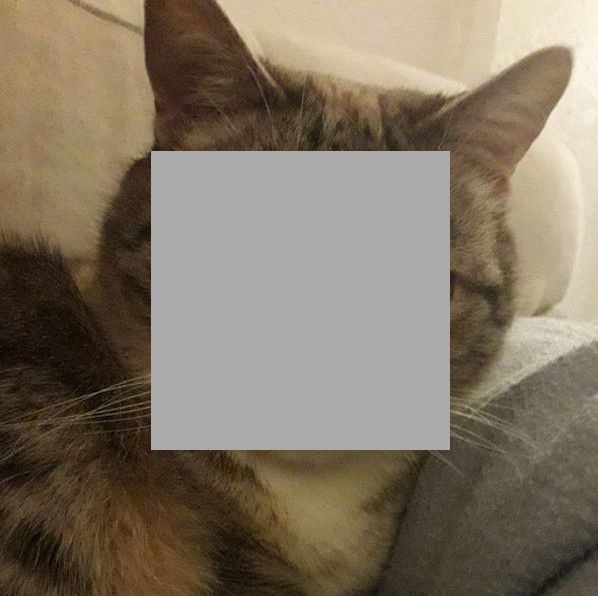
\includegraphics[width=3cm]{wendy_inpainting}
		\caption{Inpainting\\input}
		\label{fig:inpainting}
	\end{subfigure}\begin{subfigure}[t]{0.25\textwidth}
	\centering
	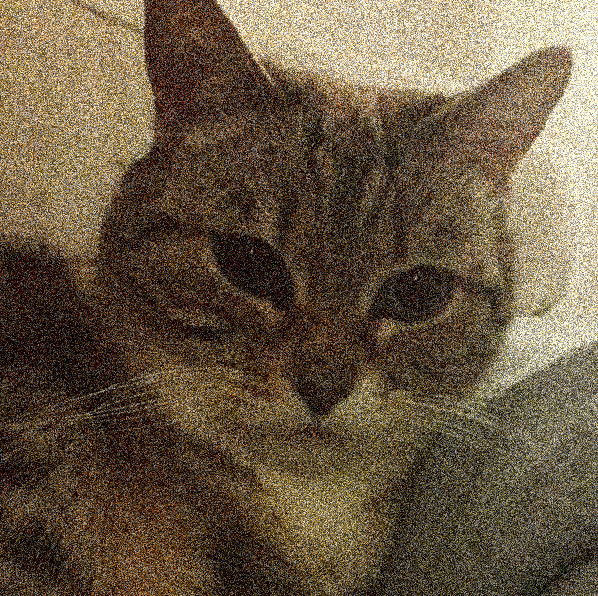
\includegraphics[width=3cm]{wendy_denoising}
	\caption{Denoising\\input}
	\label{fig:denoising}
	\end{subfigure}\begin{subfigure}[t]{0.25\textwidth}
		\centering
		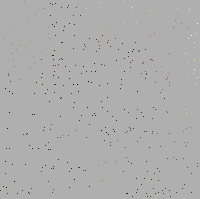
\includegraphics[width=3cm]{wendy_reconstruction}
		\caption{Reconstruction\\input}
		\label{fig:pixelwise_gen}
	\end{subfigure}
	\caption[Inpainting and image reconstruction]{Difference between regular image inpainting (\ref{fig:inpainting}), image denoising (\ref{fig:denoising}) and the problem undertaken in this work (\ref{fig:pixelwise_gen}) on the real sample depicted in sub-figure (\ref{fig:digit}).}
	\label{fig:image_completion_task}
\end{figure}


Image reconstruction belongs to the family of problems consisting in retrieving an image from an altered one. This includes problems such as inpainting \citep{Bertalmio2000} (\citefig{fig:inpainting}) or image denoising  \citep{Goyal2020} (\citefig{fig:denoising}) which consists in retrieving missing or altered parts of an image. Image inpainting (\citefig{fig:inpainting}) is the task  of recreating missing or damaged regions of an image. This kind of alterations have numerous applications, from the restoration of damaged pictures \citep{Oliveira2001} to semantic image editing \cite{Bau2019} including for example object removal \citep{Criminisi2004}. In the same fashion, image denoising (\citefig{fig:denoising}) aims to remove alterations induced by some noise, which can be due to imperfections in the acquisition procedure or natural degradation, which finds applications such as raw image denoising in cameras \citep{Kim2014} or medical image denoising \citep{Gondara2016}.

Image reconstruction (\citefig{fig:pixelwise_gen}) however differs from these problems as most part of the original image is unavailable. Thus, in comparison to inpainting or denoising in which the altered parts of the input can be retrieved from a semantically rich altered image, image reconstruction instead requires to generate a full image from very few and unstructured observations. This can be done by leveraging on prior knowledge to train a generative model, while ensuring that the resulting image is coherent with the pixels given as input.

Before delving into the details, let introduce the notations related to the problem.  Note that we use the matrix and vector formulations interchangeably, as most of the computation remains similar regardless of the number of dimensions. We denote by $\mx$ a random variable and $\vx \in \spaceR^{n\times p\times c}$ its realization. Let $\p{\mx}$ be the distribution  measure of $\mx$ over $\spaceX$. Similarly $\p{\mx|\my}$ represents the distribution of $\mx$ conditioned on the random variable $Y$, while $\p{\mx,\my}$ represents the joint distribution. 

Whether it is for image inpainting, denoising or reconstruction, we aim to recover a signal from which we only have altered measurements. This problem can be formulated as 
%
\begin{equation}
	\label{eq:reconstruction_system}
	\vy = \ma\vx + \epsilon \enspace,
\end{equation}
%
where  $\ma \in \mathbb{R}^{a\times b}$ is a wide ($a \ll b$), matrix (so called ``measurement matrix'') and $\epsilon$ is the noise. By varying the nature of the matrix $\ma$, we can formulate the three aforementioned problems.

In the case of image reconstruction, assume $\vy$ is the given set of constrained pixel values. To ease the presentation, let consider $\vy$ as a $n\times p$ image with only a few available pixels (less than $1\%$ of $n\times p$). We will encode the spatial location of these pixels using a corresponding binary mask $\mm_\vy \in \{0,1\}^{n\times p}$.  

Having access to a set of ground-truth images $ \setX = \{\vx_1,...\vx_s\}, \vx_i \in \spaceR^{n\times p\times c}$  (see Figure \ref{fig:digit}) drawn from an unknown distribution $\p{\mx}$ and a set of sparse matrices \\$  \setY = \{\vy_1,...,\vy_t\}, \vy_i \in \spaceR^{n\times p\times c}$ (Figure \ref{fig:pixelwise_gen}) as the given constrained pixels, the image reconstruction problem consists in finding an approximated image $\Hat{\vx}$ that maximizes $\p{\mx}(\Hat{\vx})$ for a given constraint map $\vy$. In other words, the problem consists in retrieving $\vx$ such that $\vy = \mm_\vy \odot \vx$ and $\vx$ is issued from to the data distribution $\p{\mx}$. More formally, we aim at finding
%
\begin{equation}
	\label{eq:formulation_IR_problem}
	\vx^* = \arg\max_\vx \p{X}(\vx) \enspace \text{subject to} \enspace \|\vy -  \mm_\vy \odot \vx\|^2_2 \leq \delta
\end{equation}
%
\noindent where $\odot$ stands for the Hadamard (or point-wise) product\footnote{Note that this expression can be formulated with the Hadamard product instead of a matrix product in \citeq{eq:reconstruction_system}, since $\vect(\mm_\vy\odot \vx) = \text{Tr}(\text{Diag}(\vect(\mm_\vy))\vect(\vx))$. $\vect(\cdot)$ is the vectorisation operator that consists in stacking the pixels, with $\vect(\vy) \in \spaceR^{n.m.c}$ for $\vy \in \spaceR^{n\times m\times c}$,  Tr($\cdot$) is the trace of a matrix and Diag($\cdot$) is an operator which transforms a vector $\vx$ into a diagonal matrix with $\vx$ as its diagonal entries.}, $\| \mn \|_2^2 $ represents the squared Frobenius norm of matrix $\mn$ that is the sum of its squared entries, $\delta$ is a small constant and $\mm_\vy$ the mask, a sparse matrix with entries equal to one at constrained pixels location. 

\section{Approaches for image reconstruction}
\label{sec:related_work}

We propose here an overview of some of the seminal approaches for solving similar tasks. We present two main types of approaches: compressed sensing-based approaches and conditional modeling. We detail some strengths and weaknesses of these approaches, summarized  in Table \ref{tab:reconstruction_approaches}. 

\subsection{Sparsity-based approaches for image reconstruction}

A first approach to tackle the image reconstruction problem is to recover the image through per-sample optimization. Although the original problem (\citeq{eq:reconstruction_system}) is linear, it is highly under determined, thus it induces an infinite number of solutions as the problem is  ill-posed. However, by including prior knowledge on the signal $\vx$ and by ensuring some constraints on the matrix $\ma$, solving this system can be done using techniques such as linear programming.

\subsubsection{Image reconstruction using compressed sensing}

\citet{Candes2005} introduced \textbf{Compressed Sensing}, which consists in solving problem (\ref{eq:reconstruction_system}) by assuming that the signal $\vx$ to be recovered is sparse. In order to guarantee that the obtained image is indeed a reconstruction, they introduced the Restricted Isometry Property (\ac{RIP}) \citep{Candes2008} on the family of matrices $\ma$, which states that for two samples $\vx_1,\vx_2 \sim \p{X}$, 
%
\begin{equation}	
	\label{eq:rip}
	(1 - \alpha)\|\vx_1 - \vx_2\|_2^2 \leq \|\ma(\vx_1 - \vx_2)\|_2^2 \leq (1 + \alpha) \|\vx_1 - \vx_2\|_2^2 \enspace,
\end{equation}
%
where $\alpha$ is a small constant. This states that distance between two samples is preserved when altered by $\ma$. \citet{Candes2005} used this property to show that if the matrix $\ma$ enforces the \ac{RIP}, samples $\Hat{\vx}$ retrieved by compressed sensing will follow with a high probability the real data distribution $\p{\mx}$. Examples of matrices that enforce the \ac{RIP} are random Gaussian or Fourier matrices \citep{Candes2006, Candes2006a}. Under the RIP setting, the sparse signal $\vx$ can be retrieved by solving for
%
\begin{equation}
	\label{eq:compressed_sensing_ell0}
	\Hat{\vx} = \arg\min_\vx  \|\vx\|_0 \enspace \text{subject to} \enspace \ma\vx = \vy \enspace .
\end{equation}
%
when the measurement process is assumed to be noiseless. In practice, the measurements processes are nearly always noisy, thus this problem must be reformulated as
%
\begin{equation}
	\label{eq:noiseful_compressed_sensing}
	\Hat{\vx} = \arg\min_\vx  \|\vx\|_0\enspace \text{subject to} \enspace \|\ma\vx - \vy\|^2_2 \leq \delta \enspace  .
\end{equation}
%
with $\delta$ a small constant. This assumes that the reconstruction is the best possible while taking noise into account. In either cases, solving this problem is NP-hard due to the $\ell_0$ norm,  however a convex relaxation seeks the minimal $\ell_1$-norm solution is also the sparsest solution \citep{Donoho2006a}. Thus we can instead recover the sparse signal $\vx$  as
%
\begin{equation}
	\label{eq:compressed_sensing}
	\Hat{\vx} = \arg\min_\vx  \|\vx\|_1 \enspace \text{subject to} \enspace \|\ma\vx - \vy\|^2_2 \leq \delta \enspace  .
\end{equation}

This method raises three important issues, the first one being that, in practice, the assumption of sparsity on $\vx$ is usually not enforced, especially for natural images.  The second problem of this approach is that it requires to solve an optimization problem for each sample. Even if the compressed sensing approach allows for the problem to be formulated as linear or quadratic programming, which can be solved in polynomial time,  it is still computationally expensive. Finally, the third issue is that the measurement matrix $\ma$ does not necessarily respect the \ac{RIP}. This is detrimental since the \ac{RIP} guarantees the coherency of the reconstructed sample. However, verifying that the matrix $\ma$ respects the \ac{RIP} is NP-hard in general. While several approaches for image compression use techniques for generating random matrices that have a high probability of respecting the \ac{RIP} \citep{Rudelson2008,Rauhut2010}, there are no guarantees in the case when $\ma$ is fixed, such as image reconstruction.

\subsubsection{Compressed sensing with sparse coding}

When aiming to recover high-dimensional signals such as natural images, the assumption of sparsity on $\vx$ is unrealistic. This requirement can however be replaced by the more generic approach of considering sparsity in another basis. Let  $\mb$ be a basis such that $\vx = \mb\vs$  and $\vs$ a sparse vector. Thus, the problem becomes 
%
\begin{equation}
	\label{eq:compressed_sensing_basis}
	\Hat{\vs} = \arg\min_\vs  \|\mb\vs\|_1 \enspace \text{subject to} \enspace \|\ma\mb\vs - \vy\|^2_2 \leq \delta \enspace  .
\end{equation}

Signal is then recovered as $\Hat{\vx} = \mb\Hat{\vs}$. By either carefully selecting $\mb$, such as Fourier or wavelet basis \citep{Mallat2008}, \textbf{compressed sensing with sparse basis} \citep{Shaobing1994} is much more robust and provides good results in real-world situations, for example in medical imaging \citep{Lustig2008}, image acquisition \citep{Kolev2011, Duarte2008}.

Another category of approaches is \textbf{dictionary learning for compressed sensing} \citep{Tosic2011}, learns the basis $\Hat{\mb}$ as a dictionary using a dataset of samples $\setX = \{\vx_1,...,\vx_K\}, \vx_i \in \spaceR^{n\times m \times c}$ such that $\vx_i = \Hat{\mb}\vs_i$, where $\vs_i$ is sparse. This can be formulated as solving for
%
\begin{equation}
	\label{eq:dictionnary_learning_ell0}
	\Hat{\mb},  \{\Hat{\vs}_i\} = \arg\min_{\mb, \{\vs_i\}} \sum_{i=1}^{K} \|\mb\vs_i - \vx_i\|^2_2  + \lambda \|\vs_i\|_0 \enspace ,
\end{equation}
%
where $\lambda$ is a parameter that controls the trade-off between the quality of the reconstruction and the sparsity of the representation. Again, solving this problem is NP-hard thus, in practice, we relax the  $\ell_1$-norm solution and solve
%
\begin{equation}
	\label{eq:dictionnary_learning}
	\Hat{\mb} = \arg\min_{\mb, \{\vs_i\}} \sum_{i=1}^{K}\ \|\mb\vs_i - \vx_i\|^2_2  + \lambda \|\vs_i\|_1 \ \enspace .
\end{equation}

This learned basis $\Hat{\mb}$ can then be used as a basis for compressed sensing. Several algorithms exist for solving this problem, usually by iteratively updating the basis $\Hat{\mb}$ and the representations $\vs_i$ alternatively. Examples of such algorithms are  LASSO \citep{Tibshirani1996}, basis pursuit \citep{Donoho2006} the method of optimal directions \citep{Engan1999},  K-SVD \citep{Aharon2006}, stochastic gradient descent or the Lagrange dual method.

\subsubsection{Generative modeling as a prior to compressed sensing}

Compressed sensing-based methods for image reconstruction have the advantage of explicitly modeling the constraints, which ensures that they will be enforced in the reconstructed image. However, there are no guarantees on the quality of the reconstruction procedure if the measurement matrix $\ma$ does not satisfy the \ac{RIP} \citeq{eq:rip}. In the case of the image reconstruction process, this means that while the reconstructed image $\hat{\vx}$ is guaranteed to enforce the constraints, it may not be necessarily close to the real data distribution $\p{X}$.

To overcome these problems, \textbf{Compressed Sensing with Meta-Learning} \citep{Wu2019} extends compressed sensing by replacing the sparsity assumptions on the signal $\vx$ with a learned prior on the data distribution $\p{X}$, which is done using a generative model $\G$.  By first generating an image $\G(\vz)$ in an unconstrained way and optimizing in the latent space $\spaceZ$ of the generative model $\G$ by minimizing $\|\ma\G(\vz) - \vy\|^2_2$, this method finds an image that, when altered as $\Hat{\vy}=\ma\G(\vz)$ where $\Hat{\vy}$, is as close as possible to $\vy$. Then, Compressed sensing with meta-learning trains the generative model $\G$ to enforce the \ac{RIP} (\citeq{eq:rip}) so that it does not try to map all $\G(\vz)$ into the null space of $\ma$. The overall problem induced by this approach is formulated as
%
\begin{align}
	\label{eq:csmeta}
	\min_\G L(\G) = \mathop{\mathbb{E}}_{\substack{\vx\sim \p{X}\\\vy\sim \p{Y}\\\vz\sim \p{Z}}} \Big( &\big(\|\ma(\vx - \G(\vz))\|_2^2  - \|\vx -\G(\vz)\|^2_F\big)^2   + \big(\|\ma(\vx - \G(\Hat{\vz}))\|_2^2  - \|\vx -\G(\Hat{\vz})\|^2_2\big)^2  \nonumber \\
	&  + \big(\|\ma(\G(\vz) - \G(\Hat{\vz}))\|_2^2  - \|\G(\vz) -\G(\Hat{\vz})\|^2_F\big)^2 \Big) / 3 	+ \|\vy - \ma\G(\hat{\vz}) \|^2_2 \nonumber \\
	&\text{where } \hat{\vz} = \min_\vz \|\vy - \ma\G(\vz) \|^2_2\enspace.
\end{align}

The method tries to minimize the difference between the distances among samples (generated or real) and the distances among samples altered by $\ma$. Solving this problem pushes the generator towards producing samples on which the \ac{RIP} of $\ma$ is respected. This implies that the generated samples will have a high likelihood on the real data distribution. Note that, in practice, $\hat{\vz}$ is computed with gradient descent on $\vz$ by minimizing $\|\vy - \ma\G(\vz) \|^2_2$, starting from a random $\vz \sim \p{Z}$. \\


\textbf{Deep Compressed Sensing} \citep{Wu2019} extends even further compressed sensing by replacing the (usually random) measurement matrix $\ma$ in the Compressed sensing with Meta-Learning approach by a learned measurement function $f_\theta$, so that the altered sample becomes $\tilde{\vy} = f_\theta(\vx)$. Then, Deep Compressed sensing consists in training, in the same fashion as the \ac{GAN} algorithm, $\G$ and $f_\theta$ by alternate gradient descent. The induced optimization problem is therefore
%
\begin{align}
	\label{eq:dcs}
	\min_\G L_{\G} &= \mathop{\mathbb{E}}_{\substack{\vy\sim \p{Y}}} \ \|\vy - f_\theta(\G(\Hat{\vz}))\|^2_2 \enspace,\\
	\label{eq:dcs_a}
	\min_\theta L_{f_\theta} =& \mathop{\mathbb{E}}_{\substack{\vx\sim \p{X}\\\vz\sim \p{Z}}} \Big( \sum_{\substack{\vx_1, \vx_2 \in \setX\cup \{G(\vz)\} \\\vx_1 \ne \vx_2}}((\|f_\theta(\vx_1 - \vx_2)\|_2^2  - \|\vx_1 -\vx_2\|^2_2)^2 \Big) \enspace.
\end{align}

In the same fashion as the objective in \citeq{eq:csmeta}, solving problem (\ref{eq:dcs_a}) pushes $f_\theta$ towards respecting the \ac{RIP}. \citet{Wu2019} showed that optimizing these two criterions trains both the generator $\G$ and the measurement function $f_\theta$, thus replacing the discriminator of the more classical \ac{GAN} framework.  As a benefit, the approach may generate an image $\hat{\vx} = \G(\hat{\vz})$ from a noisy information $\vy$ but at a high computation burden since it requires to solve an optimization problem (computing $\hat{\vz}$) at inference stage for generating an image.
%and so that $\tilde{y}$ is as close as possible to $\vy$. %the sparsity assumption on the signal $\vx$ a learned prior on the data distribution $\p{X}$, as a generative model $\G$.  By first generating an image $\G(\vz)$ and exploring the latent space $\setZ$ of the generative model $\G$ by minimizing $\|A\G(\vz) - \vy\|^2_2$, so that altering the generated image gives $\Hat{\vy}=A\G(\vz)$ where $\Hat{\vy}$ is as close as possible to $\vy$. Then, Compressed sensing with meta-learning trains the generative model $\G$ to enforce the \ac{RIP} (\citeq{eq:rip}) so that it does not try to map all $\G(\vz)$ into the null space of $\ma$. The overall problem induced by this approach is formulated as

% 		\begin{multline}
% 	    	\min_G L(G) = \mathop{\mathbb{E}}_{\substack{x\sim \p{X}\\y\sim \p{Y}\\z\sim \p{Z}}} \Big[\Big( (\|f_\theta (x - \G(z))\|_2^2 - \|x - \G(z)\|_2^2)^2 + (\|f_\theta (x - \G(\hat{z}))\|_2^2 - \|x - \G(\hat{z})\|_2^2)^2 \\
% 	    	+ (\|f_\theta (G(z) - \G(\hat{z}))\|_2^2 - \|G(z) - \G(\hat{z})\|_2^2)^2 \Big) / 3
% 	    	+ \|y - f_\theta(G(\hat{z})) \|^2_2\Big]\\
% 	    	\text{where } \hat{z} = \min_z \|y - f_\theta(G(z)) \|^2\enspace.
% 		\end{multline}


%where $\setS$ contains the three samples $\vx, \G(\vz), \G(\hat{\vz})$. 
%In practice, $\hat{\vz}$ is computed with gradient descent on $\vz$ by minimizing $\|\vy - AG(\vz) \|^2_2$, and starting from a random $\vz \sim \p{Z}$. As a benefit, this approach may generate an image $\hat{\vx} = \G(\hat{\vz})$ from a noisy information $\vy$ but again at a high computation burden since it requires to solve an optimization problem (computing $\hat{z}$) at inference stage for generating an image.



\subsection{Conditional generation for image reconstruction}
\label{subs:conditional_reconstruction}

\begin{figure}[t]
	\centering
	\begin{subfigure}[t]{0.25\textwidth}
		\centering
		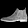
\includegraphics[scale=1.5]{origin.png}
		\caption{Original\\Image}
		\label{fig:original_shoe}
	\end{subfigure}\begin{subfigure}[t]{0.25\textwidth}
		\centering
		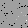
\includegraphics[scale=1.5]{consts.png}
		\caption{Constraints}
		\label{fig:constraints}
	\end{subfigure}\begin{subfigure}[t]{0.25\textwidth}
		\centering
		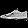
\includegraphics[scale=1.5]{img.png}
		\caption{Generated\\Image}
		\label{fig:pixelwise}
	\end{subfigure}\begin{subfigure}[t]{0.24\textwidth}
		\centering
		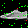
\includegraphics[scale=1.5]{imgcolor.png}
		\caption{Satisfied\\Consts.}
		\label{fig:generated}
	\end{subfigure}
	\caption[Generation of a sample during training]{Generation of a sample during training. We first sample an image from a training set (\ref{fig:original_shoe}) and we compute the constraints (\ref{fig:constraints}) from it. Our GAN uses it to generate a sample (\ref{fig:pixelwise}). The constraints with squared error smaller than $\epsilon=0.1$ are deemed satisfied and shown by green pixels in (\ref{fig:generated}) while the red pixels are unsatisfied (Best viewed in colors).}
	\label{fig:image_completion}
\end{figure}

As opposed to the aforementioned methods, approaches based on conditional generation try to learn the conditional distribution $\p{X|Y}$ with a set of samples $\setX = \{\vx_1,...\vx_s\}$ and either aims to generate the most probable solution or provide a sampling mechanism over potential solutions. 

In the case of image reconstruction, a generative model $\G$ which input is constraint map $\vy \in  \spaceR^{n\times p\times c}$ learns to generate an image satisfying the constraints while likely following the distribution $\p{X}$ (see \citefig{fig:image_completion}). For a generative model to provide a sampling mechanism, the common solution consists in relying on  a random vector $\vz$  sampled from a known distribution $\p{Z}$ (usually uniform or  Gaussian) over a space $\spaceZ$ that will be used as a latent variable for the model.

\subsubsection{Conditional generative adversarial networks for image reconstruction}

Although \ac{CGAN} was initially designed for class-conditioned image generation by setting $\vy$ as the class label of the image, it can naturally be applied to several types of conditioning information, including constraint maps. Thus obtaining an  image reconstruction with a high likelihood on the conditional distribution $\p{X|Y}$ is equivalent to taking a sample or image $\Hat{\vx} = \G(\vy, \vz)$, with $\vz \sim \p{Z}$, using the generative model $\G$ solution to the problem
%
\begin{equation}
	\label{eq:CGAN_problem_reco}
	\min_\G\max_\D \esp{\vx,\vy\sim \p{X,Y}} [\log \D(\vx, \vy)] +  \esp{\vy\sim \p{Y} \\ \vz\sim\p{Z}} [1 - \log \D(\G(\vy, \vz), \vy)] \enspace ,
\end{equation}
%
where $\vy$ is the constraint map and $\D$ is the discriminator network.

While using the \ac{CGAN} approach alone could theoretically be enough to solve the tasks of image reconstruction and inpainting, as it directly learns the conditional distribution of the samples, the most efficient approaches rely on extending the \ac{CGAN} with a reconstruction loss, such as a $\ell_1$ or $\ell_2$ norm, between the pixels known beforehand and the corresponding pixels in the generated sample. This has been carried out for the inpainting task \citep{Pathak2016, Xiang2017}, and can be formulated (in the case of the $\ell_2$ norm) as finding a generator $\G$ and related discriminator $\D$ that optimize
%
\begin{equation}
	\label{eq:CGAN_problem_reco_norm}
	\min_\G\max_\D \esp{\vx,\vy\sim \p{X,Y}} [\log \D(\vx, \vy)] +  \esp{\vy\sim \p{Y} \\ \vz\sim\p{Z}} [1 - \log \D(\G(\vy, \vz), \vy)] +  \| \mm_\vy \odot \G(\vy, \vz) - \vy \|^2_F \enspace .
\end{equation}
%
These approaches are often extended with techniques such as using multiple discriminators \citep{Yu2018, Armanious2019}, extending the training with extra information and features \citep{Armanious2019} as for medical imaging modalities, or using style losses \citep{Guo2019} (See \citesec{subs:augmented_objectives}). However, several of these CGAN-based inpainting methods \citep{Demir2018} rely on generating a patch that will fill up a structured missing part of the image and achieve impressive results. As such, they are not well suited to reconstruct from very sparse and unstructured observations $\vy$. 

\subsubsection{Unsupervised image reconstruction with generative adversarial networks}

Another trend of approaches aims to reconstruct images without any knowledge of the real data distribution $\p{X}$, in other words they only hinge on datasets of altered samples $\vy \sim \p{Y}$. This problem is different from the one we tackle, since ours supposes that a dataset of unaltered samples $\setX = \{\vx_1, ...,  \vx_s\}, \vx_i \in \spaceR^{n\times m\times c}$ is available.  Among these approaches is \textbf{Ambient \ac{GAN}} \citep{Bora2018} (Figure \ref{fig:ambientgan}), which aims at training an unconditional generative model using a dataset of noisy or incomplete samples $\setY=\{\vy_1,...\vy_t\}, \vy_i\in \spaceR^{n\times m\times c}$. Ambient \ac{GAN} attempts to produce unaltered images $\tilde{\vx}$ which distribution matches the true one without having access to any of the original images $\vx$. For the sake, Ambient \ac{GAN} considers lossy measurements such as a blurred image, an image with removed patch or removed pixels at random (up to 95\%), leading to sparse pixel map $\vy$. This lossy measurement is simulated with a parameterized alteration function $f_\theta$ instead of the measurement matrix $\ma$
%
\begin{equation}
	\label{eq:denoising_system}
	\vy = f_\theta(\vx) \enspace.
\end{equation}
%
The underlying optimization problem solved by Ambient \ac{GAN} is therefore stated as
%
\begin{equation}
	\label{eq:ambientgan}
	\min_G \max_D L(D, G) = \mathop{\mathbb{E}}_{\substack{\vy\sim \p{Y}}} \Big[\log(\D(\vy))\Big] + \mathop{\mathbb{E}}_{\substack{\vz\sim \p{Z} \\\theta \sim p_\theta}} \Big[ \log(1-\D(f_\theta(\G(\vz))))\Big] \enspace.
\end{equation}
%
Here, the discriminator has no knowledge of the distribution of the full images $\p{X}$, as its input is either real altered samples $\vy$ or generated samples $G(\vz)$ on which the alteration function $f_\theta$ is applied. Thus, the Ambient GAN generator network $\G$ actually learns to generate samples $\Hat{\vx} = \G(\vz)$ that, once$f_\theta$ is applied on them, are close to the real $\vy$. This is equivalent to learning to invert the function $f_\theta$. The Ambient GAN process is described in \citefig{fig:ambientgan}.\\

\begin{figure}
	\centering
	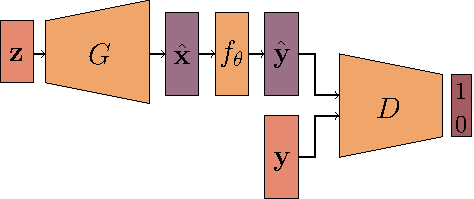
\includegraphics[width=(\textwidth/3)*2]{ambientgan.pdf}
	\caption[Overview of the Ambient GAN framework]{Overview of the \textbf{Ambient GAN} framework for learning generative models using altered samples only.}
	\label{fig:ambientgan}
\end{figure}


\textbf{Unsupervised Image Reconstruction} (\ac{UNIR}) \citep{Pajot2019} extends the Ambient GAN approach by adding a conditioning to the model, which allows for the reconstruction of an image $\vx$ from an altered image $\vy\sim\p{Y}$, without any knowledge of the real data distribution $\p{X}$. \ac{UNIR} is deterministic and does not allow for sampling, as the only input of the model is the altered image $\vy$. For this, an additional reconstruction task is considered. It consists in first generating a reconstruction $\tilde{\vx} = \G(\vy)$ and applying the alteration function $f_\theta$ to the generated image $\tilde{\vx}$ to get $\tilde{\vy} = f_\theta(\G(\vy))$, then re-generating an image as $\hat{\vx} = \G(f_\theta(\G(\vy)))$ and finally re-applying $f_\theta$ to the image $\Hat{\vx}$ to get $\Hat{\vy} = f_\theta(\G(f_\theta(\G(\vy))))$. This procedure can be deemed as 
%
\begin{equation}
	\label{eq:unir}
	\min_\G \max_\D L(\D, \G) = \mathop{\mathbb{E}}_{\substack{\vy\sim \p{Y}}} \Big[\log(\D(\vy))\Big] + \mathop{\mathbb{E}}_{\substack{\vy\sim \p{Y} \\\theta \sim p_\theta}} \Big[ \log(1-\D(\hat{\vy}))\Big] + \|\hat{\vy} - \tilde{\vy} \|^2_F \enspace.
\end{equation}
\noindent
Here, the $\ell_2$ norm term ensures that the generator is able to learn to revert $f_\theta$ i.e. to revert the alteration procedure on a given sample. This  allows the reconstruction of a realistic image $\Hat{\vx}$ only from a given constraint map $\vy$. The full process is described in \citefig{fig:unir}.

\begin{figure}
	\centering
	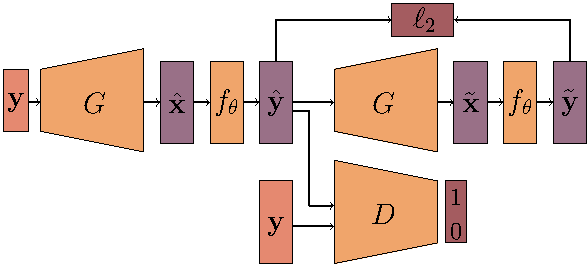
\includegraphics[width=\textwidth]{unir.pdf}
	\caption[Overview of the Unsupervised Image Reconstruction framework]{Overview of the \textbf{Unsupervised Image Reconstruction} framework for learning image reconstruction  models using altered samples only.}
	\label{fig:unir}
\end{figure}


In another fashion, \textbf{Semantic Inpainting by Constrained Image Generation} \citep{Yeh2017} is an approach for inpainting which considers the generator $\G$ of a pre-trained \ac{GAN} as a prior on the data distribution $\p{X}$, and explores its latent space $\spaceZ$ through an optimization procedure to find a latent vector $\vz$, which induces an image with missing regions filled in by conditioning on the surrounding available information. To ensure that the reconstruction is accurate, this approach uses the discriminator $\D$ as a prior instead of ensuring the \ac{RIP}. This is done by adding the discriminator loss to the reconstruction loss, so that it prevents the procedure from providing images that are too far away from the real data distribution. As such, the problem becomes $\Hat{\vx} = \G(\vz^*)$ with $\vz^*$ minimizing
%
\begin{align}
	\label{eq:semantic_inpainting}
	\min_\vz \|\ma\G(\vz) &- \vy \|^2_2 +  \lambda \log(1 - \D(\G(\vz))) \enspace ,
\end{align}
%
where $\lambda$  is a hyperparameter. To yield on an image satisfying some given constraints $\vy$, the method requires to solve a full optimization problem for each sample to reconstruct.

A summary of the main features of the presented related work is provided in Table \ref{tab:reconstruction_approaches}. These features are the need for a dataset of samples, with only the need for altered samples for the Ambient GAN and UNIR approaches; the need for solving a reconstruction problem for each generated image,  which is computationally expensive; the ability to sample multiple images on the conditional distribution $\p{Y|X}$ for a given $\vy$, and the different ways to control the enforcement of the constraints.

\begin{table}
	\centering
	\begin{tabular}{|l|c|c|c|c|}
		\hline
		\textbf{Approach} & \textbf{Dataset} & \textbf{One-step}   		& \textbf{Sampling}  &      \textbf{Constraint}s\\
		 				  					 & \textbf{free}  & \textbf{reconstruction} & \textbf{mechanism}&	 \textbf{enforcement}\\  															  
		\hline
    	\hline
		\multicolumn{5}{|l|}{\textbf{Compressed sensing-based}} \\
		\hline
		\hline
		Compressed sensing			   & \cmark & \xmark & \xmark & Exact \\
		\citep{Candes2005} 				&                 &				 &				&			  \\
		\hline
		Compressed sensing 				 &             & 				&				&  \\ 							
	    with dictionary learning 	& \xmark & \xmark & \xmark &  Exact \\
	     \citep{Donoho2006}				 &             & 				&				&   \\
  		\hline
	    Compressed sensing                 &             & 				&				& 	Control	   \\
	    with Meta Learning 	               & \xmark & \xmark  &\xmark   &	parameter				   \\
	    \citep{Wu2019} 	                         &              &			   &			    & \\
		\hline
		 Deep compressed sensing    & \xmark & \xmark  &\cmark & Control\\
		\citep{Wu2019}						    &              &				  &			   & parameter\\
		\hline
		\hline
		\multicolumn{5}{|l|}{\textbf{Generative modeling-based}} \\
		\hline
		\hline
		Conditional GAN 										  &  \xmark & \cmark & \cmark & Implicit \\
		\citep{Mirza2014} 										&   			 &				 &				&			        \\
		\hline
		Ambient GAN 									   			  & \xmark & \xmark & \xmark    & Explicit\\
		\citep{Bora2018} 										&  (altered*) &				 &			      &			    \\
		\hline
		UNIR   									   			  				 & \xmark & \cmark & \xmark    & Explicit \\
		\citep{Pajot2019} 										& (altered*) &				 &			      &			   \\
		\hline
		Constrained                  								&             & 				&				& 	Control	   \\
		image generation              							& \xmark & \xmark  &\cmark   &	parameter				   \\
		\citep{Yeh2017} 	                         				&              &			   &			    & \\
		\hline
		\hline
		\textbf{Our approach}   							& \xmark & \cmark & \cmark    & Control \\
		(see Section \ref{sec:our_approach})&              &				  &			   & parameter\\
		\hline
	\end{tabular}
	{\begin{flushleft}\footnotesize* Only altered samples are required during training\end{flushleft}}
%
	\caption[Approaches for image reconstruction]{Summary of the advantages and limitations of the aforementioned methods for image reconstruction. We consider the need for a dataset, the necessity of solving an optimization problem for each generated sample, the ability to sample different solutions and the mechanism for enforcing the good reconstruction of the constraints.}
	\label{tab:reconstruction_approaches}
\end{table}

\section{Image reconstruction as an auxiliary task to generative modeling}
\label{sec:our_approach}

 As we have seen, two main categories of solutions aim to tackle the problem of image reconstruction. First, the approaches that try to directly solve the problem by finding a solution through optimization, among them is compressed sensing. However, the main drawback of these approaches are that they require to solve an optimization problem per reconstructed image, which is computationally expensive in the cases where a lot of samples need to be reconstructed. Then, the approaches that aims to learn the conditional data distribution $\p{X|Y}$ to reconstruct the image by sampling on this distribution. Among these approaches are \ac{CGAN}-based methods, Ambient GAN or UNIR. While they have the advantage of only requiring to solve a unique optimization problem at training instead of one for each reconstructed sample, they require a dataset to train on and do not provide any means of controlling the trade-off between the visual quality and the respect of the constraints.

As  a main contribution in this chapter, we introduce a \ac{GAN} model whose generation network takes as input the constraint map $\vy$ and the sampled latent code $\vz \in \spaceZ$ and outputs a realistic image that fulfills the prescribed pixel values. Within this setup, such a generative model can sample in a single step from the unknown distribution $\p{X}$ of the training images $\{\vx_1, \cdots, \vx_N\}$ while satisfying unseen pixel-wise constraints at training stage.  This method also provides a control parameter $\lambda$ that balances the visual quality and the respect of the constraints.

\subsection{Image reconstruction as a maximum a posteriori estimation}

Starting from the image reconstruction problem ((\citeq{eq:reconstruction_system}), estimating the maximum a posteriori consists in finding an image $\Hat{\vx}$ that has the maximum likelihood on the posterior distribution $\p{X|Y}$, in other words the image that is the most likely to be the original image, from which the constraints $\vy$ has been measured. We find that replacing the implicit conditioning of the \ac{CGAN} with a reconstruction loss is an approach that naturally emerges from the denoising formulation \citeq{eq:denoising_system}. This provides a rationale for the use of these losses in the similar aforementioned approaches (\citesec{subs:conditional_reconstruction}). 
 
 Such a generative model does not rely on per-sample optimization and provides a simple and efficient sampling mechanism through the latent variable $\vz$. This allows for the efficient sampling of several potential images, which can be crucial in some applications in which a large amount of solutions need to be sampled, such as solving inverse problems \citep{Laloy2019} . It also naturally provides a mechanism for controlling the trade-off between the respect of the constraints and the likelihood of the reconstructed image.
 
\subsubsection{Conditional generative models for maximum a posteriori estimation}
\label{subs:maximum_a_posteriori}

Recall that the image reconstruction problem consists in recovering $\vx$, assuming the constraint map $\vy$ is resulting from applying $\mm_\vy$ on the image $\vx$, as
%
\begin{equation}
\vy = \mm_\vy \odot\vx \enspace.
\label{eq:noiseless_generation_primary_CGAN}
\end{equation}
%
Here $\mm_\vy$ is the masking matrix and the constrained pixels are assumed to be randomly and independently selected.  We can formulate the Maximum A Posteriori (MAP) estimation problem which, given the constraint map $\vy$, consists in finding the most probable image $\vx^*$ following the posterior distribution $\p{X|Y}$, as
%
\begin{align}
\vx^* &= \arg\max_\vx\log {\p{X|Y}}(\vx|\vy) + \log \p{Y}(\vy)\enspace,\\
&= \arg\max_\vx\log \p{Y|X}(\vy|\vx)+ \log \p{X}(\vx) \enspace.
\label{eq:bayesian_formulation_our_primary_CGAN}
\end{align}

$\p{Y|X}(\vy|\vx)$ is the likelihood that the constrained pixels $\vy$ are issued from image $\vx$ while $\p{X|Y}(\vx|\vy)$ is the likelihood of an image knowing the constrained pixels $\vy$ . $\p{X}$ and $\p{Y}$ represent the marginal distributions of $\vx$ and $\vy$. Thus, we can introduce a conditional generative model $\G : (\spaceY, \spaceZ) \rightarrow \spaceX$ to replace the conditional distribution $\p{X|Y}$. This changes the original problem (\citeq{eq:noiseless_generation_primary_CGAN}) to
%
\begin{equation}
	\vy = \mm_\vy \odot \G(\vy, \vz) + \epsilon \enspace,
	\label{eq:generation_primary_CGAN}
\end{equation}
%
where $\epsilon$ represents the error of the model, which we consider to be an i.i.d noise corrupting the constrained pixels. Assuming that the generation network $\G$ may sample an image $\G(\vy, \vz)$ complying with the given pixel values $\vy$, we get the following problem

\begin{equation}
	\max_G \mathop{\mathbb{E}}_{\substack{\vy\sim \p{Y}\\\vz\sim \p{Z}}} \log \p{Y|X}(\vy| \G(\vy, \vz)) + \log \p{X}(\G(\vy, \vz)) \enspace.
\label{eq:bayesian_formulation_our_primary_CGAN_G}
\end{equation}

he first term in Problem (\ref{eq:bayesian_formulation_our_primary_CGAN_G}) measures the likelihood of the constraints given a generated image. The second term measures the likelihood of the generated images according to the data distribution $\p{X}$. Let rewrite Equation (\ref{eq:bayesian_formulation_our_primary_CGAN_G}) as $\vect(\vy) = \vect(\mm_\vy \odot \vx) + \vect(\varepsilon)$ where $\vect(\cdot)$ is the vectorisation operator that consists in stacking the pixels, with $\vect(\vy) \in \spaceR^{n.m.c}$ for $\vy \in \spaceR^{n\times m\times c}$. Therefore, assuming $\vect(\varepsilon)$ is i.i.d and follows a Gaussian distribution $\mathcal{N}(0,\sigma^2 I)$, the conditional likelihood of $\vy$ knowing $\vx$  reads as
\begin{equation}
\log \p{Y|X}(\vy, \G(\vy| \vz)) \, \propto - \left \|\vect(\vy) - \vect(\mm_\vy \odot \G(\vy,\vz))\right\|_2^2 \enspace.
\end{equation}
\noindent It evaluates the euclidean distance between the conditioning pixels and their predictions by $\G$. In other words, using a matrix notation of  Equation (\ref{eq:generation_primary_CGAN}), the latter conditional likelihood given a generated image equivalently writes

\begin{equation}
\log {p_{Y|X}}(\vy, \G(\vy, \vz) \, \propto - \left \|\vy - \mm_\vy \odot \G(\vy,\vz)\right\|_F^2 \enspace.
\end{equation}
%
%In this work, we assume that $\epsilon$ follows a normal distribution $\epsilon\sim\mathcal{N}[0,\sigma^2]$, but it is worth noting that any prior distribution with a close-form solution for maximum likelihood estimation (typically distribution from the exponential family) can be used.
%In the case of the normal distribution, we can minimize our error term by using the $L_2$ norm on the constrained pixels.
%    

The second term in Problem (\ref{eq:bayesian_formulation_our_primary_CGAN_G}) is the likelihood of the generated image under the true but unknown data distribution $\p{X}$. Maximizing this term can be equivalently achieved by minimizing the distance between $\p{X}$ and the marginal distribution of the generated samples $\G(\vy,\vz)$. This amounts to minimizing with respect to $\G$, the GAN-like objective function $\mathop{\mathbb{E}}_{\substack{\vx\sim \p{X}}} \log(\D(\vx)) + \mathop{\mathbb{E}}_{\substack{\vz\sim \p{Z}\\\vy\sim \p{Y}}} \log(1-\D(\G(\vy, \vz)))$  \citep{Goodfellow2014}.

\clearpage

Putting altogether these elements, we can propose a relaxation of the hard constraint optimization problem (\ref{eq:formulation_IR_problem}) (Figure \ref{fig:ourapproach}) that consists in learning a generative network $\G$ and the related discriminator model $\D$ by solving
%minimizing the Jensen-Shannon divergence between the real data distribution and the distribution of the generated data \citep{Goodfellow2014}.

%In our approach, we explicitly model the relaxation of the constraint by minimizing the $L_2$ norm between the constrained pixels and the generated values (see Fig.\ref{fig:ourapproach}).

%The objective function, with $\lambda \geq 0$ an additional parameter, becomes:
\begin{eqnarray}
\min_\G \max_\D L(\D,\G) & {\small=} & \mathop{\mathbb{E}}_{\substack{\vx\sim \p{X}}} \Big[\log(\D(\vx))\Big] \label{eq:final_optim_problem} \\
&+&\mathop{\mathbb{E}}_{\substack{\vz\sim \p{Z}\\\vy\sim \p{Y}}} \Big[\log(1-\D(\G(\vy, \vz)))+\lambda \left\|\vy - \mm_\vy \odot \G(\vy,\vz)\right\|_F^2 \Big] \enspace . \nonumber
\end{eqnarray}

\begin{figure}
	\centering
	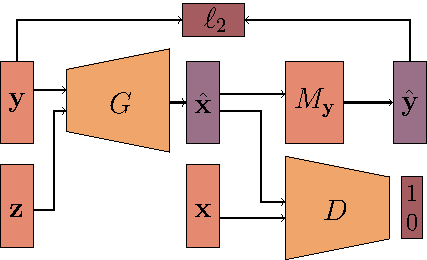
\includegraphics[width=(\textwidth/3)*2]{ours.pdf}
	\caption[Maximum  a posteriori \ac{GAN} for image reconstruction]{Overview of our formulation of the maximum  a posteriori approach for image reconstruction using \ac{GANs}.}
	
	\label{fig:ourapproach}
\end{figure}


It is worth to note that the assumption of Gaussian noise measurement leads us to explicitly turn the pixel value constraints into the  minimization of the quadratic error between the real enforced pixel values and their generated counterparts as it corresponds to maximizing the conditional likelihood of the pixels in the generated  image. The additional term acts as a regularization over prescribed pixels by the mask $\mm_\vy$. The trade-off between the distribution matching loss and the constraint enforcement is assessed by the regularization parameter $\lambda \geq 0$. Figure \ref{fig:ourapproach} illustrates the overall principle of the model. It is also worth noting that the noise $\varepsilon$ can be of any other distribution, according to the prior information one may associate to the measurement noise. To formulate the maximum a posteriori, we however require this distribution to admit a closed-form solution for the maximum likelihood estimation for optimization purpose. Typical choices are distributions from the exponential family \citep{Brown1986}.

\subsubsection{Conditional image generation with an image reconstruction auxiliary task}

To solve Problem (\ref{eq:final_optim_problem}), we use stochastic gradient descent. The overall training procedure is detailed in Algorithm \ref{alg:train} and ends up when a maximal number of training epochs is attained. 

\begin{algorithm}[!ht]
	\caption{Proposed training algorithm}
	\label{alg:train}
	\begin{algorithmic}[H]
		\REQUIRE{ $\trainsetX$ the set of  unaltered images, $\G$ the generation network, and $\D$ the discrimination function}
		\REPEAT
		\STATE sample a mini-batch $\lbrace \vx_i \rbrace_{i=1}^m$ of real images from $\trainsetX$\;
		\STATE sample a mini-batch of masks $\lbrace \mm_{\vy_i} \rbrace_{i=1}^m$ and compute the constraints $\vy_i = \mm_{\vy_i} \odot \vx_i$\;
		\STATE sample a mini-batch $\lbrace \vz_i \rbrace_{i=1}^m$ from distribution $\p{Z}$ \;
		\STATE update $\D$ by stochastic gradient ascent of
		\STATE \ \ \ \ $ \sum_{i=1}^{m}\log(\D(\vx_i)) + \log(1-\D(\G(\vy_i, \vz_i)))$
		\STATE sample a mini-batch $\lbrace \vy_j \rbrace_{j=1}^n$ from $\trainsetY$\;
		\STATE sample a mini-batch $\lbrace \vz_j \rbrace_{j=1}^n$ from distribution $\p{Z}$\;; 
		\STATE update $\G$ by stochastic gradient descent of
		\STATE \ \ \ \ $ \sum_{j=1}^n \log(1-\D(\G(\vy_j, \vz_j))) + \lambda\|\vy_j - \mm_{\vy_j}\odot \G(\vy_j, \vz_j)\|_F^2$\;
		\UNTIL a stopping condition is met
		
	\end{algorithmic}
\end{algorithm}

When implementing this training procedure we experienced, at inference stage, a lack of diversity in the generated samples (see Figure \ref{fig:diversity_loss}). This issue manifests itself through the fact that the learned generation network, given a constraint map $\vy$, outputs almost deterministic image  regardless the variations in the input $\vz$. The issue was also pointed out by Yang et al. \citep{Yang2019} as characteristic of \ac{CGAN}s. To avoid the problem, we exploit the PacGAN \citep{Lin2018} technique, detailed in \citesec{subs:augmented_objectives},  which consists in passing a small set of samples to the discrimination function instead of a single one.  PacGAN is intended to tackle the mode collapse problem in GAN training (see \citesec{subs:mode_collapse}) . The underlying principle being that if a set of images are sampled from the same training set, they are very likely to be completely different, whereas if the generator experiences mode collapse, generated images are likely to be similar. In practice, we only give two samples to the discriminator, which is sufficient to overcome the loss of diversity as  suggested in \citep{Lin2018}. The resulting training procedure is summarized in Algorithm~\ref{alg:trainpac}.

\begin{figure}[h]
	\centering
	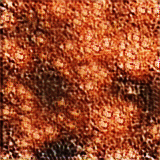
\includegraphics[width=2cm]{diversity_1.png}\hspace{0.5cm}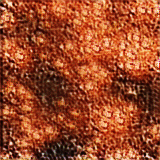
\includegraphics[width=2cm]{diversity_2.png}\hspace{0.5cm}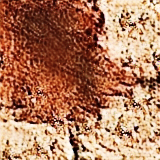
\includegraphics[width=2cm]{diversity_1_pac.png}\hspace{0.5cm}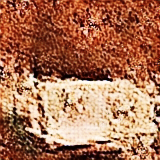
\includegraphics[width=2cm]{diversity_2_pac.png}
	
	\vspace{0.3cm}
	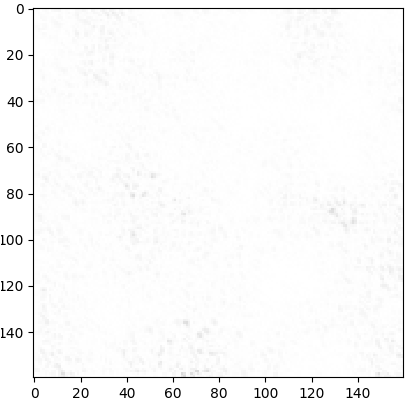
\includegraphics[height=4cm]{diversity_diff_nobar.png}\hspace{0.5cm}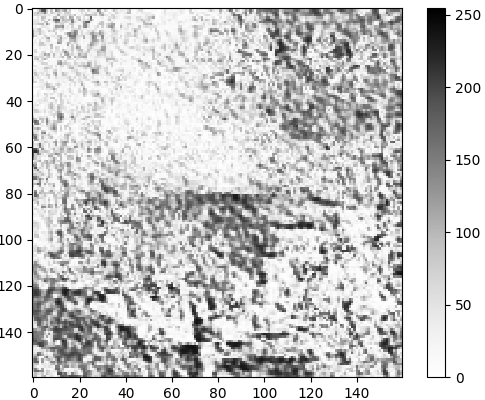
\includegraphics[height=4cm]{diversity_diff_pac.png}
	\caption[An example of a loss of diversity]{An example of a loss of diversity when generating brick texture samples (see \citesec{sec:experiments_protocol}) using two different random noises $\vz$ and a single constraint map $\vy$. The two samples on the top left are generated using the classical GAN discriminator whereas the samples on the top right are generated using the PacGAN approach. The loss of diversity is clearly visible on the absolute differences between the greyscaled images (bottom).}
	\label{fig:diversity_loss}
\end{figure}

\begin{algorithm}[]
	\caption{Our training algorithm including PacGAN}
	\label{alg:trainpac}
	\begin{algorithmic}[H]
		\REQUIRE { $\trainsetX$ the set of  unaltered images, $\G$ the generation network, and $\D$ the discrimination function}
		\REPEAT
		\STATE sample two mini-batches $\lbrace \vx_i^a \rbrace_{i=1}^m$, $\lbrace \vx_i^b\rbrace_{i=1}^m$ from $\trainsetX$\;
		\STATE sample a mini-batch of masks $\lbrace \mm_{\vy_i} \rbrace_{i=1}^m$ and compute the constraint maps $\{\vy_i = \mm_{\vy_i} \odot \vx_i^a\}$\;
		\STATE sample two mini-batches $\lbrace \vz_i^a \rbrace_{i=1}^m$, $\lbrace \vz_i^b \rbrace_{i=1}^m$ from distribution $\p{Z}$ \;
		\STATE update $\D$ by stochastic gradient ascent of
		\STATE \ \ \ \  $ \sum_{i=1}^{m}\log(\D(\vx_i^a, \vx_i^b)) + \log(1-\D(\G(\vy_i, \vz_i^a), \G(\vy_i, \vz_i^b)))$
		\STATE sample a mini-batch of masks $\lbrace \mm_{\vy_i} \rbrace_{i=1}^m$ and compute the labels $\vy_i = \mm_{\vy_i} \odot \vx_i$\;
		\STATE sample a mini-batches $\lbrace \vz_i^a \rbrace_{i=1}^m$, $\lbrace \vz_i^b \rbrace_{i=1}^m$ from distribution $\p{Z}$ \;
		\STATE update $\G$ by stochastic gradient descent of
		\STATE \  $ \sum_{j=1}^m \log(1-\D(\G(\vy_j, \vz_j^a), \G(\vy_j, \vz_j^b))) + \lambda\|\vy_j - \mm_{\vy_j}\odot \G(\vy_j, \vz_j^a)\|_F^2  + \lambda\|\vy_j - \mm_{\vy_j}\odot \G(\vy_j, \vz_j^b)\|_F^2$\;
		\UNTIL a stopping condition is met
		
	\end{algorithmic}
\end{algorithm}


\FloatBarrier

\subsection{Experimental results and application}
\label{sec:experiments}

\subsubsection{Experimental setting} \label{sec:experiments_protocol}
We have conducted a series of empirical evaluation to assess the performances of the proposed GAN. Used datasets, evaluation protocol and the tested deep architectures are detailed in this section while Section \ref{subs:results} is devoted to the results presentation. We compare our approach to the \ac{CGAN} approach exclusively, as it is the only approach among the methods reviewed in Section \ref{sub:image_reconstruction_problem} to provide a sampling  mechanism while not requiring to solve a computationally expensive optimization problem for each generated sample (see Table \ref{tab:reconstruction_approaches}). 
\subsubsection{Datasets}
We tested our approach on several datasets listed hereafter. Detailed  information on these datasets are provided  in the Appendix \ref{app:det_datasets}.
%namely FashionMNIST \citep{Xiao2017}, CIFAR10 \citep{Krizhevsky2009CIFAR10}, CelebA\citep{liu2015celeba} and a custom-made Texture texture dataset:
\begin{description}
	\item{FashionMNIST} \citep{Xiao2017} consists of 60,000 $28\times 28$ small gray-scale images of fashion items, split in 10 classes and is a harder version of the classical MNIST  dataset \citep{LeCun1998a}. %known to be simple to solve. 
	The very small size of the images makes them particularly appropriate for large-scale experiments, such as hyper-parameter tuning. 
	
	\item{CIFAR10} \citep{Krizhevsky2009} consists of 60,000 $32 \times 32$ color images of 10 different and varied classes. It is deemed less easy than MNIST and FashionMnist.
	%considered harder to learn that MNIST and FashionMNIST, even it is of nearly the same dimension.
	\item{CelebA} \citep{Liu2015} is a large dataset of celebrity portraits labeled by identity and a variety of binary features such as eyeglasses, smiling... We use 100,000 images cropped to a size of $128 \times 128$, making this dataset appropriate for a high dimension evaluation of our approach in comparison with related work. Samples are shown in Figure \ref{fig:samples_celeba}
	
	\item{Texture} is a custom dataset 
	%was eventually created that is composed of texture, sampling $20000$ patches
	composed of $20,000$ $160 \times 160$ patches sampled from a large brick wall texture, as recommended in \citep{Jetchev2017}. It is worth noting that this procedure can be reproduced on any texture image of sufficient size. Texture is a test-bed of our approach on fully-convolutional networks for constrained texture generation task. \ref{fig:samples_texture}
	%This allows us to experiment fully-convolutional architectures on a texture reconstruction task.
	
	\item{Subsurface} is a classical dataset in geological simulation \citep{Strebelle2002} which consists, similarly to the Texture dataset, of 20,000  $160 \times 160$ patches sampled from a model of a subsurface binary domain. These models are assumed to have the same properties as a texture.  \ref{fig:samples_subsurface}
	
	
\end{description}

To avoid learning explicit pairing of real images seen by the discrimination function with constraint maps provided to the generative network, we split each dataset into training, validation and test sets, to which we add a set composed of constraint maps that should remain unrelated to the three others.
To do so, a fifth of each set is used to generate the constrained pixel map $\vy$ by randomly selecting uniformly $0.5\%$ of the pixels to compose a set of constraints for each of the train, test and validation sets. The images from which these maps are sampled are then removed from the training, testing and validation sets. For each carried experiment the best model is selected based on some performance measures (see Section \ref{subs:eval}) computed on the validation set. Finally, reported results are computed on the test set.

%To avoid learning explicit correlations between real examples presented to the discriminator and constraint maps given to the generator, we create a splitting consisting in the classical train, validation and test databases, to which we add a constraints database that should remain unrelated to the three others. A fifth of each set is used to generated the matrix of constraints $C$ by randomly selecting $0.5\%$ of the pixels, uniformly. These images are then removed from the training, testing and validation sets.


\subsubsection{Network architectures}
\label{subs:architectures}

We use a variety of neural network architectures for the \ac{GAN} generator and discriminator in order to adapt to the different scales and image sizes of our datasets. The detailed configuration of these architectures are exposed in Appendix \ref{app:det_archis}.

For the experiments on the FashionMNIST \citep{Xiao2017}, we use a lightweight convolutional network for both the discriminator and the generator, similar to \ac{DCGAN}  \citep{Radford2015}, due to the small resolution of FashionMNIST images.
%This is motivated by the large number of experiments and the small dimension of the images.

To experiment on the Texture dataset, we consider a set of fully-convolutional generator architectures based on either \gl{dilconv}{dilated convolutions} \citep{Yu2015}, which behave well on texture datasets \citep{Ruffino2017}, or \gl{encdec}{encoder-decoder} architectures that are commonly used in domain-transfer applications such as CycleGAN \citep{Zhu2017}.

We keep the PatchGAN discriminator \citep{Isola2016} across all the experiments with these architectures, which is a five-layer fully-convolutional network with a sigmoid activation.

The Up-Dil architecture consists in a set of \gl{deconv}{transposed convolutions} (the up-scaling part), and a set of dilated convolutional layers \citep{Yu2015}, while the Up-EncDec has an up-scaling part followed by an encoder-decoder section with skip-connections, where the constraints are down-scaled, concatenated to the noise, and re-up-scaled to the output size.

The UNet \citep{Ronneberger2015} architecture is an \gl{encdec}{encoder-decoder} where \gl{skip}{skip-connections} are added between the encoder and the decoder.
The Res architecture is an \gl{encdec}{encoder-decoder} where \gl{resblock}{residual blocks} \citep{He2015} are added after the noise is concatenated to the features. The UNet-Res combines the UNet and the Res architectures by including both residual blocks and skip-connections.

Finally, we will evaluate our approach on the Subsurface dataset using the architecture that yields to the best performances on the Texture dataset.

\subsubsection{Evaluation}
\label{subs:eval}

We evaluate our approach based on both the satisfaction of the pixel constraints and the visual quality of sampled images. From the assumption of Gaussian measurement noise (as discussed in Section \ref{subs:maximum_a_posteriori}), we assess the constraint fulfillment using the following mean square error (\ac{MSE}) 
\begin{equation}
MSE = \frac{1}{L} \sum_{i=1}^L \left\|\vy_i - \mm_{\vy_i} \odot \G(\vy_i, \vz_i)\right\|_F^2 \enspace.
\end{equation}
This metric should be understood as the mean squared error of reconstructing the constrained pixel values. 

Visual quality evaluation of an image is not a trivial task \citep{Theis2015}. However, Fréchet Inception Distance (\ac{FID}) \citep{Heusel2017} and Inception Score \citep{Salimans2016}, have been used to evaluate the performance of generative models. These approaches  both consist in comparing, for both real and generated images, features extracted with a pre-trained classifier. We explain these approaches in section \ref{subs:evaluation_methods} of the chapter 1. We employ \ac{FID} since the Inception Score has been shown to be less reliable \citep{Barratt2018}. Since the \ac{FID} requires a pre-trained classifier adapted to the dataset in study, we trained simple convolutional neural networks as classifiers for the FashionMNIST and the CIFAR-10 datasets. For the Texture dataset, the dataset is not labeled, hence we resort to a CNN classifier trained on the Describable Textures Dataset (DTD) \citep{Cimpoi2014}, which is a related application domain.

For the Subsurface dataset, there is not labels nor similar labeled dataset. Thus, we could not train a classifier for this dataset, so we cannot compute the FID. To evaluate the quality of the generated samples, we use metrics based on a distance between feature descriptors extracted from real samples and from generated ones. Similarly to \citep{Ruffino2017}, we rely on a $\chi^2$ distance between the Histograms of Oriented Gradients (\ac{HOG}) or Local Binary Patterns (\ac{LBP}) features computed on generated and real images. Histograms of Oriented Gradients (\ac{HOG}) \citep{Dalal2005} and Local Binary Patterns (\ac{LBP}) \citep{Pietikainen2011} are computed by splitting an image into cells of a given radius and computing within each cell the histograms of the oriented gradients for \ac{HOG}s and of the light level differences for each pixel to the center of the cell for \ac{LBP}s.  Additionally, we consider the domain-specific metric, the connectivity function \citep{Lemmens2017} which is presented in Appendix \ref{app:geostatistics}.

Finally, we check by visual inspection if the trained model $\G$ is able to generate diverse samples, meaning that for a given $\vy$ and for a set of latent codes $(\vz_1, ..., \vz_n) \sim \p{Z}$, the generated samples $\G(\vy,\vz_1), \ldots, \G(\vy, \vz_n)$ are visually different. 

%Since we empirically observed that our models were either producing very different samples or samples that only differ by a small noise factor, we do not propose a specific evaluation metric and instead check manually if a loss of diversity occurs.

\subsubsection{Study of the quality-fidelity trade-off}
\label{subs:results}

% \begin{figure}[!]
%     \centering
%     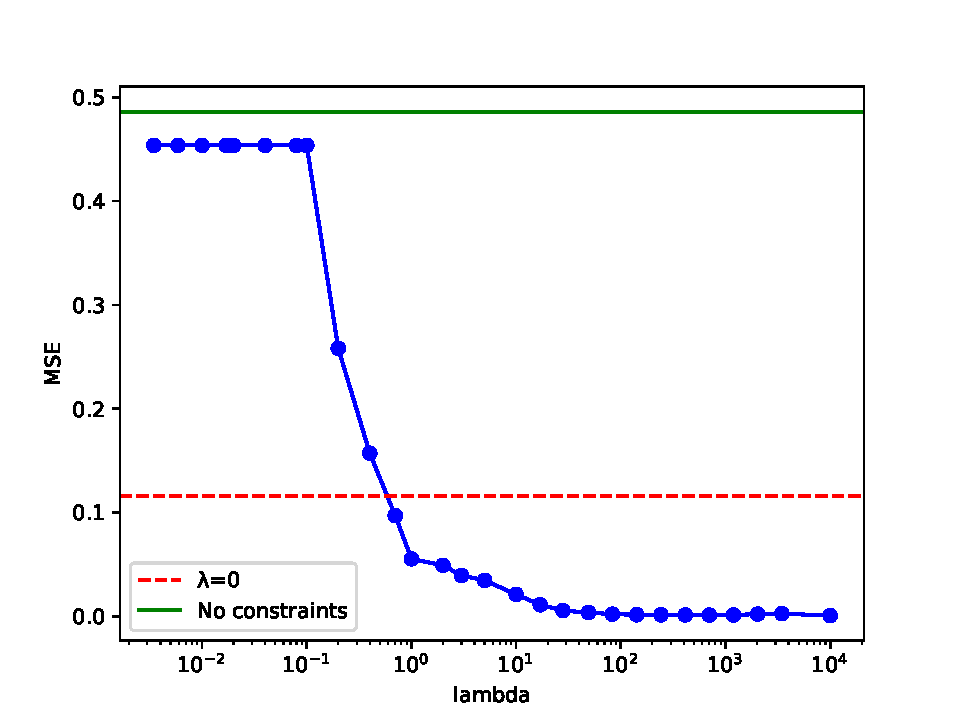
\includegraphics[trim=0 0 0 40, clip,scale=0.35]{MSE_mnist}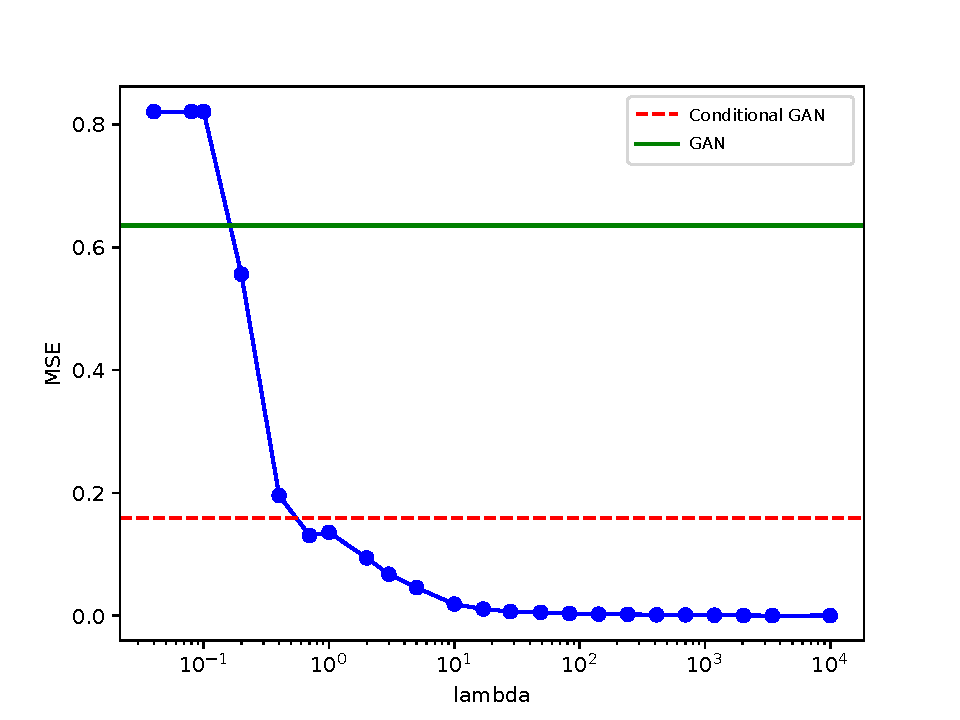
\includegraphics[trim=0 0 0 40, clip,scale=0.35]{MSE_fashion}
%     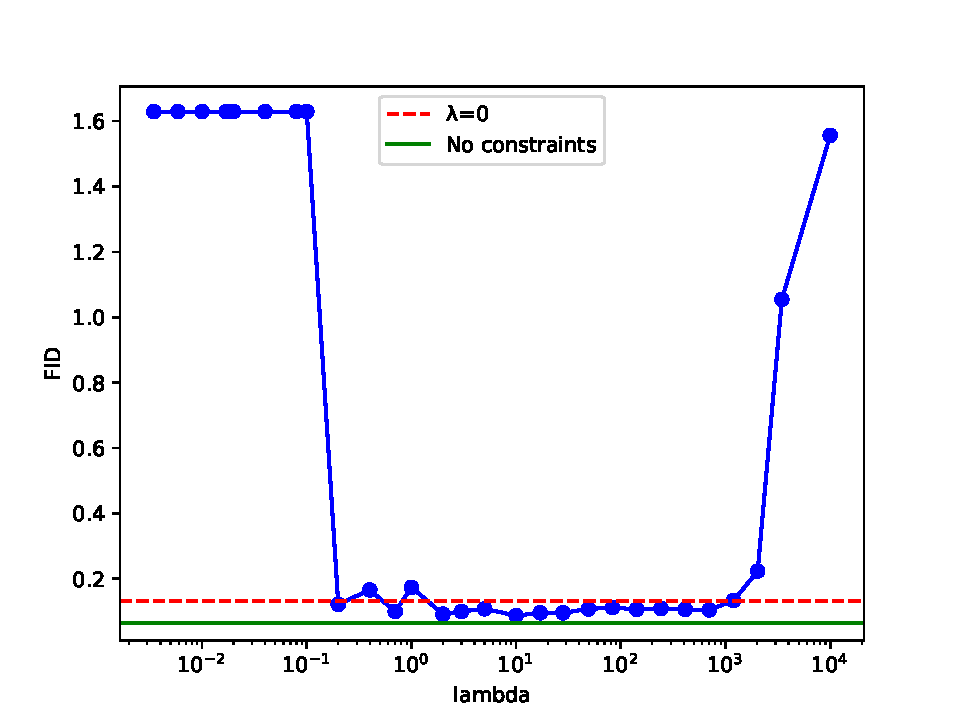
\includegraphics[trim=0 0 0 40, clip,scale=0.35]{FID_mnist}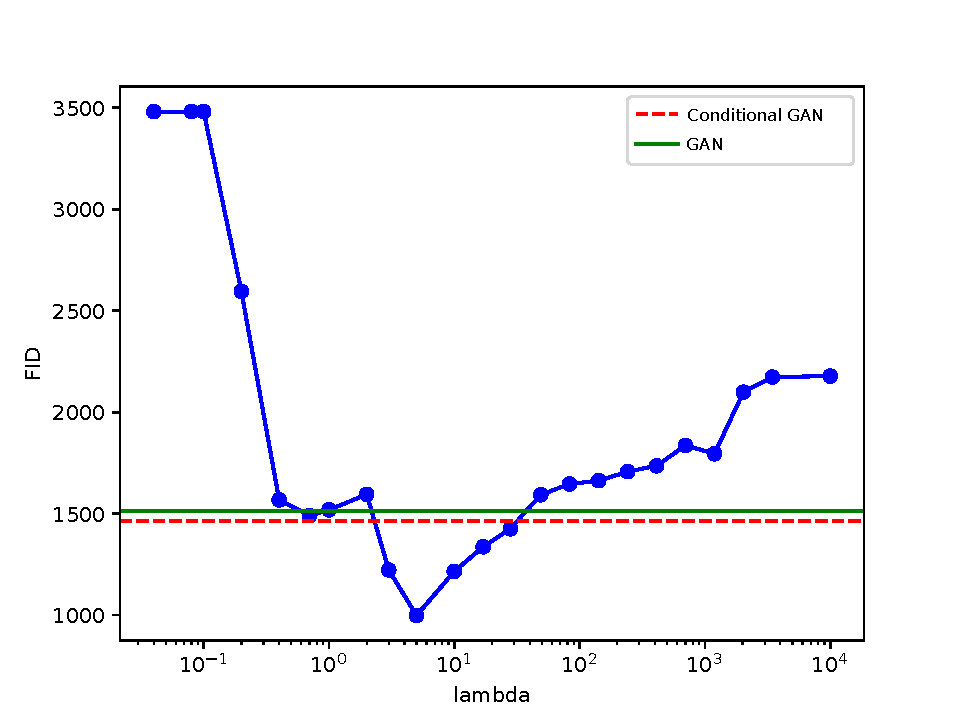
\includegraphics[trim=0 0 0 40, clip,scale=0.35]{FID_fashion}

%     \centering
%     \caption{MSE (top) and  FID (bottom) w.r.t. the regularization parameter $\lambda$;
%     Dataset MNIST (left), Fashion MNIST (right).
%     %The different orders of magnitude for the Y-axis of the FID is due to the different classifiers used to compute this distances.
%     }
%     \label{fig:fids}
%     \label{fig:mses}
% \end{figure}


%In this set of experiments, 
We first study the influence of the  regularization parameter $\lambda$ on both the quality of the generated samples and the respect of the constraints. We experiment on the %MNIST \citep{Lecun1998} and
FashionMNIST \citep{Xiao2017} dataset, since such a study requires intensive simulations permitted by the low resolution of FashionMNIST images and the used architectures (see Section \ref{subs:architectures}). 
%a lot of re-training and the small size of the images allowed us to run several hundreds of experiments.

\begin{figure}[!h]
	\begin{tabular}{ll} 
		\multicolumn{1}{c}{\hspace{-20px}\textbf{MNIST}} & \multicolumn{1}{c}{\hspace{-20px}\textbf{FashionMNIST} \hspace{20px}}\\
		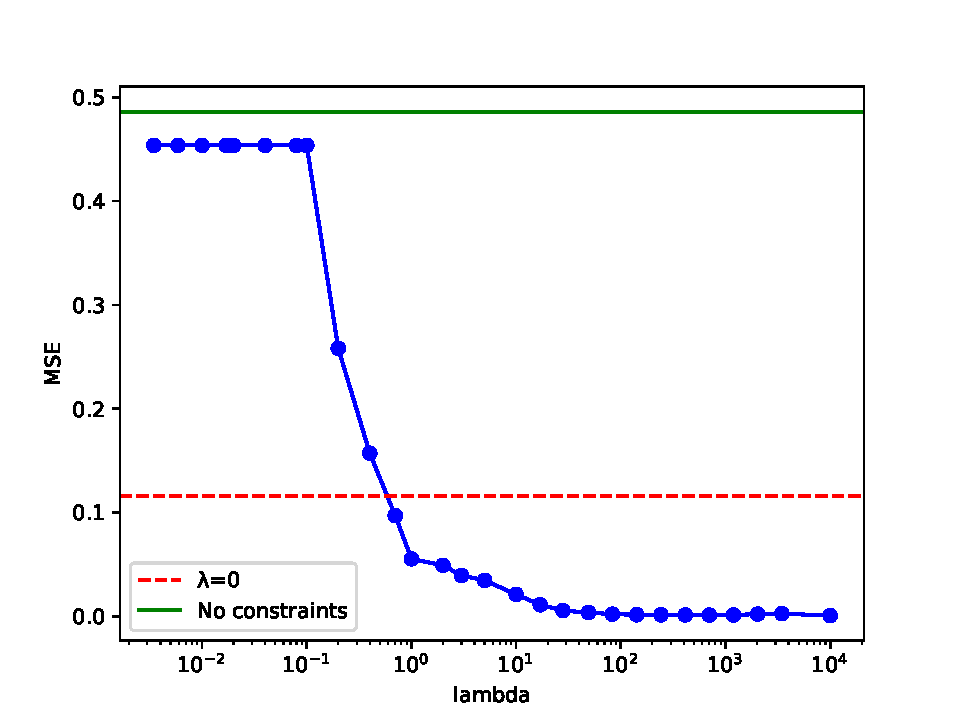
\includegraphics[trim=20 0 0 40, clip,scale=0.5]{MSE_mnist}				 & 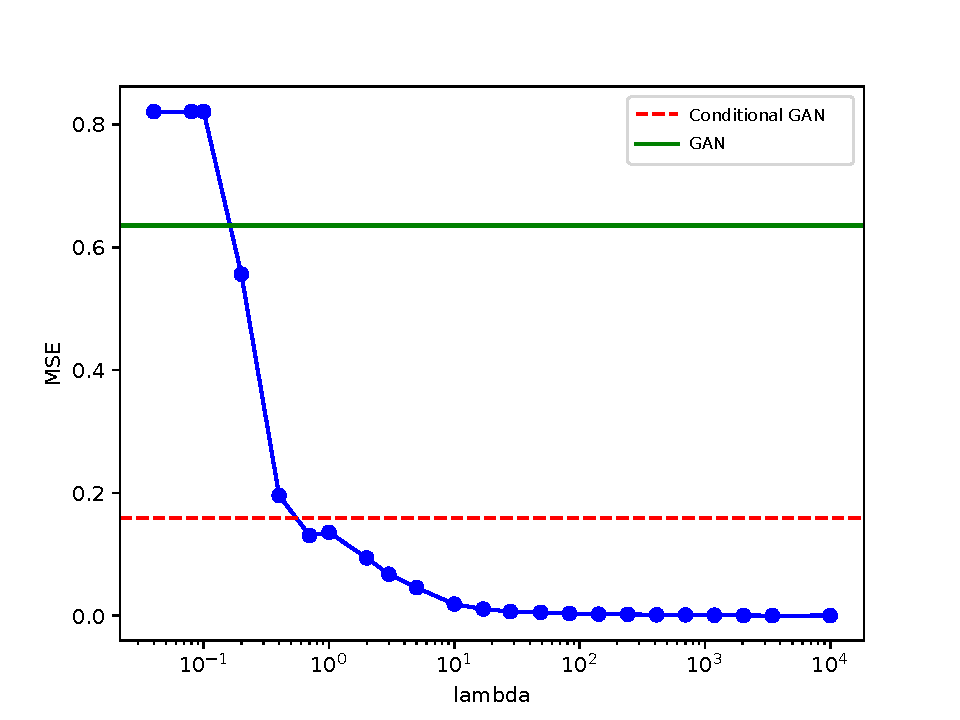
\includegraphics[trim=30 0 0 40, clip,scale=0.5]{MSE_fashion} \\
		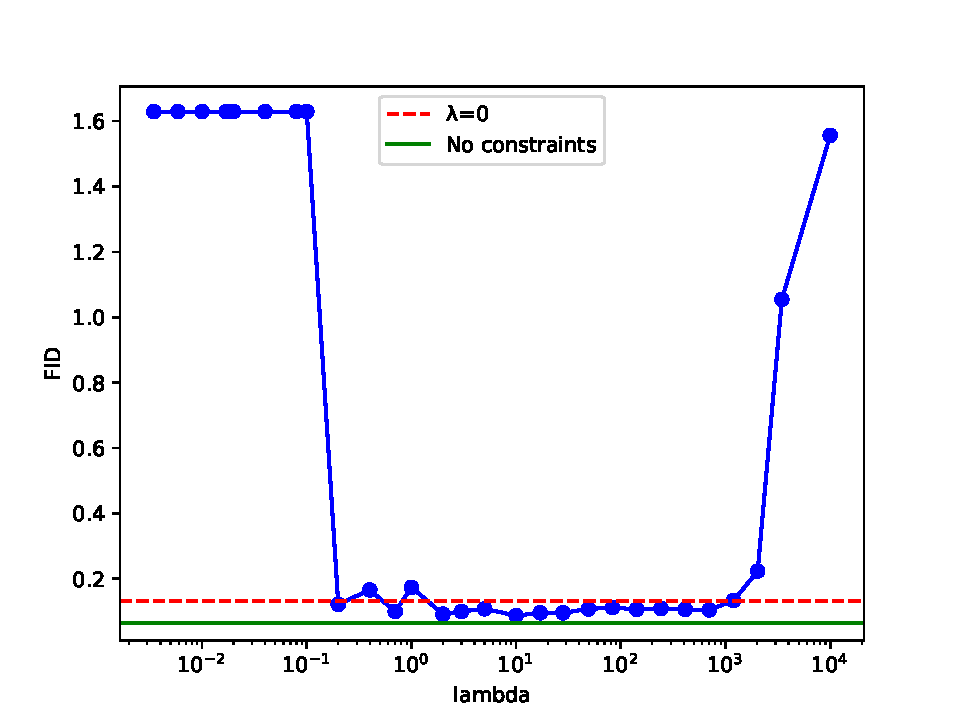
\includegraphics[trim=20 0 40 40, clip,scale=0.5]{FID_mnist}				 & 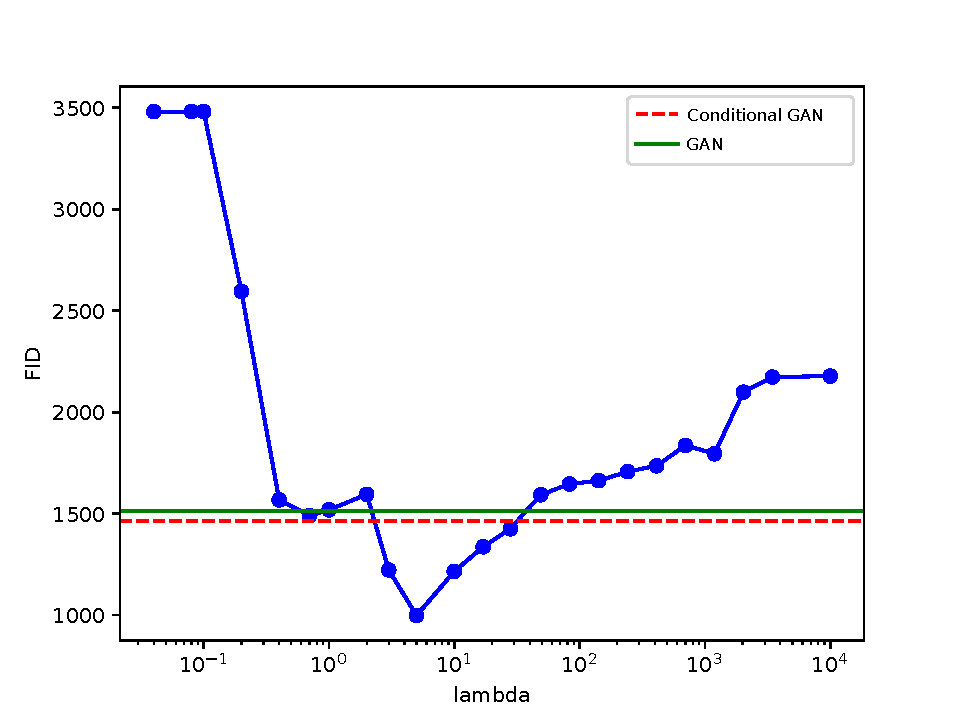
\includegraphics[trim=25 0 0 40, clip,scale=0.5]{FID_fashion} \\
		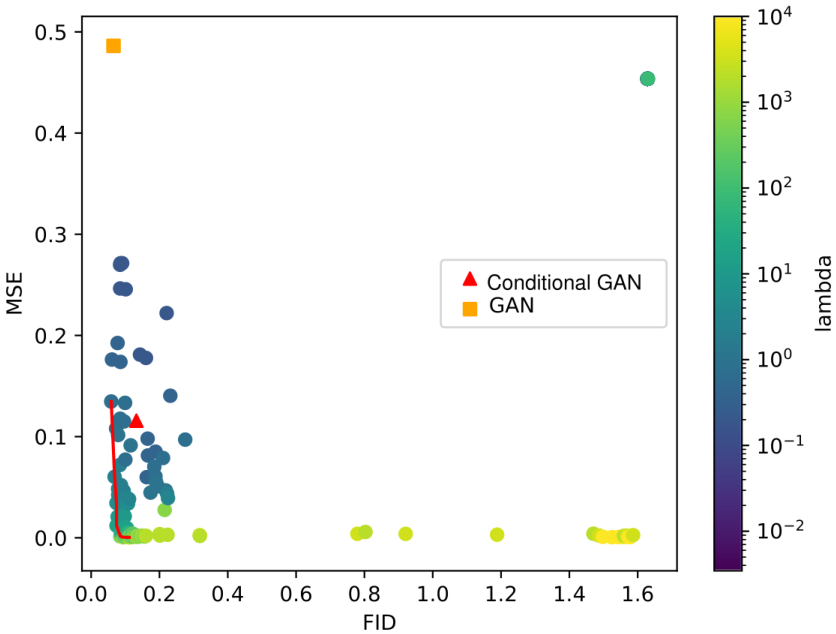
\includegraphics[trim=00 0 20 00, clip,scale=0.6]{pareto_mnist} & 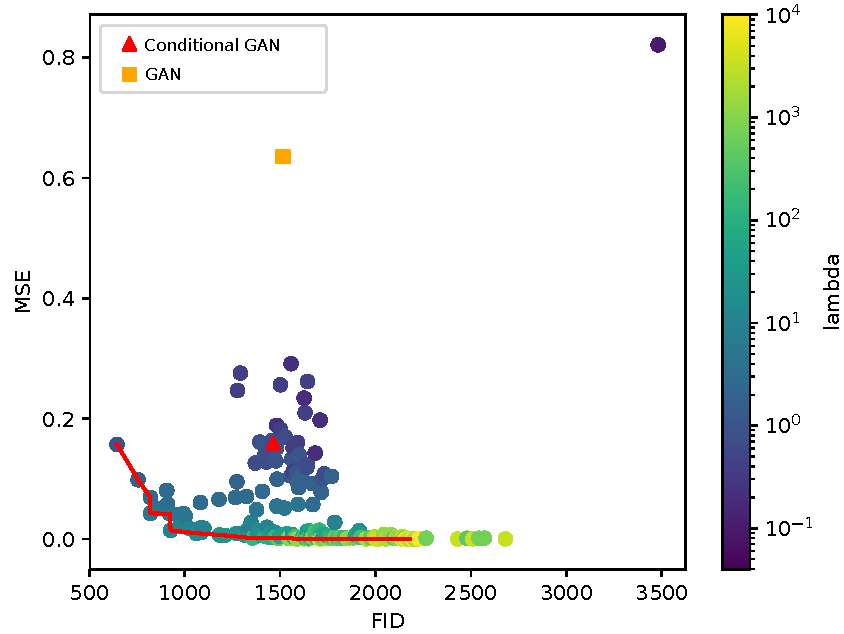
\includegraphics[trim=20 0 0 0, clip,scale=0.6]{pareto_fashion} \\
	\end{tabular}
	\caption[Hyperparameter study for our approach and GAN/CGAN on two datasets]{Our approach compared to the GAN and CGAN baselines. MSE (Top) and  FID (center) w.r.t. the regularization parameter $\lambda$; MSE w.r.t the FID (bottom), on the MNIST (left) and Fashion MNIST (right) datasets. Note  that the different orders of magnitude for the FID is due to the different classifiers used to compute this distances.
	}
	\label{fig:fids}
	\label{fig:mses}
	\label{fig:paretos}
\end{figure}

To overcome classical GANs instability, the networks are trained 10 times and the median values of the best scores on the test set at the best epoch 
are recorded. The epoch that minimizes the cost
\begin{equation*}
C(FID, MSE) = \sqrt{\left(\frac{FID - FID_{min}}{FID_{max}- FID_{min}}\right)^2 + \left(\frac{MSE - MSE_{min}}{MSE_{max}- MSE_{min}}\right)^2}
\end{equation*}  on the validation set is considered as the best epoch, where $FID_{min}$, $MSE_{min}$, $FID_{max}$ and $MSE_{max}$ are respectively the lowest and highest \ac{FID}s and \ac{MSE}s obtained on the validation set.

Empirical evidences (highlighted in Figure \ref{fig:mses}) show that with a good choice of $\lambda$, the regularization term helps the generator to enforce the constraints, leading to smaller \ac{MSE}s than when using the \ac{CGAN} ($\lambda=0$) without compromising on the quality of generated images. Also, we can note that using the regularization term even leads to a better image quality compared to \ac{GAN} and \ac{CGAN}.
%
The bottom panel in Figure \ref{fig:paretos} illustrates that the trade-off between image quality and the satisfaction of the constraints can be controlled by appropriately setting the value of $\lambda$. Nevertheless, for small values of $\lambda$ (less or equal to $10^{-1}$), our GAN model fails to learn meaningful distribution of the training images and only generates uniformly black images. This leads to the plateaus on the \ac{MSE} and \ac{FID} plots (top panels in Figure \ref{fig:mses}).



% \begin{figure}
%     \centering
%     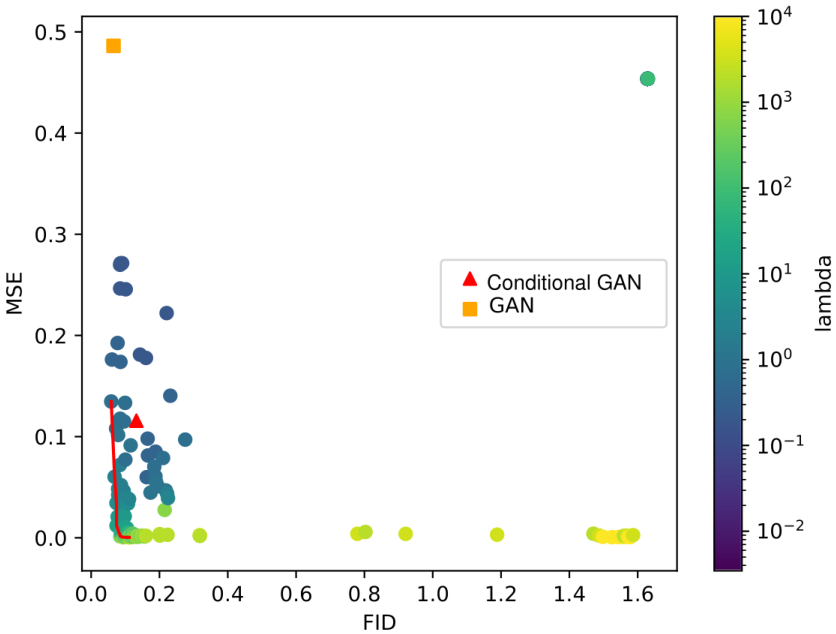
\includegraphics[trim=0 0 0 40, clip,scale=0.4]{pareto_mnist}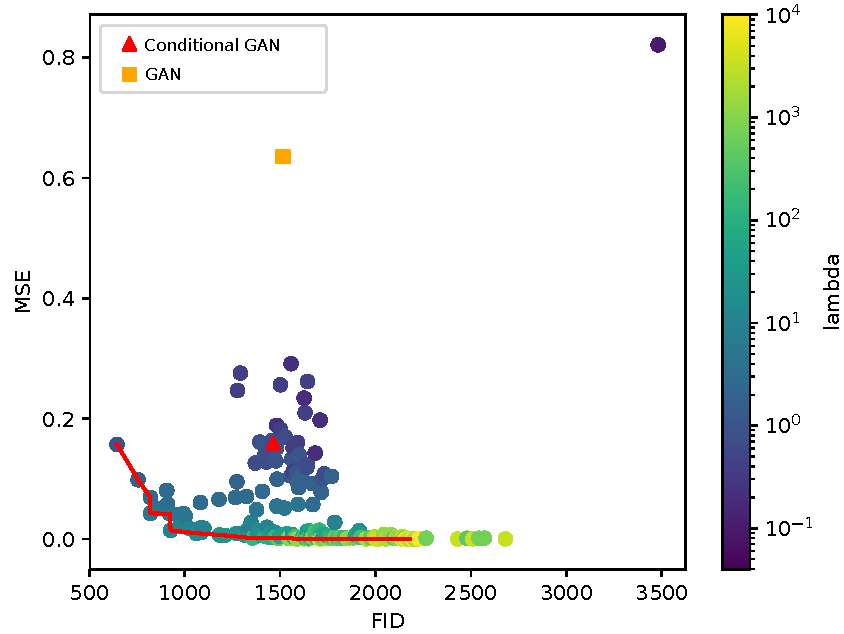
\includegraphics[trim=0 0 0 40, clip,scale=0.4]{pareto_fashion}
%     \vspace*{-3mm}
%     \caption{MSE w.r.t the FID. Left: MNIST; Right: Fashion MNIST. Note that due to the failure mode previously mentioned, a large part of the values are stacked in the top right corner of these figures.
%     }
%     \label{fig:paretos}
% \end{figure}  

\subsubsection{Texture generation with fully-convolutional architectures}
\label{sub:fcnn}
Fully-convolutional architectures for GANs are widely used, either for domain-transfer applications \citep{Zhu2017, Isola2016} or for texture generation \citep{Jetchev2017}. In order to evaluate the efficiency of our method on relatively high resolution images, we experiment the fully-convolutional networks described in Section \ref{subs:architectures} on a texture generation task using Texture dataset. We investigate the up-scaling-dilatation network, the \gl{encdec}{encoder-decoder} one and the \gl{resnet}{ResNet}-like architectures.

Our training algorithm ran for 40 epochs on all reported results. We provide a comparison to CGAN \citep{Mirza2014} approach by using the selected best architectures.
The models are evaluated in terms of best FID (visual quality of sampled images) at each epoch and MSE (conditioning on fixed pixel values).  We also compute the FID score of the models at the epochs where the MSE is the lowest. In the other way around, the MSE is reported at epoch when the FID is the lowest. The obtained performances are detailed in Table \ref{tab:ablation}.

For the \gl{encdec}{encoder-decoder} models, we can notice that the models using ResNet blocks perform better than just using a \gl{unet}{UNet} generator. A trade-off can also be seen between the FID and MSE for the ResNet models and the \gl{unet}{UNet}-ResNet, which could mean that skip-connections help the generator to fulfill the constraints but at the price of lowered visual quality.

Although the \gl{encdec}{encoder-decoder} models perform the best, they tend to lose diversity in the generated samples (see Figure \ref{fig:diversity_loss}), whereas the up-scaling-based models have high FID and MSE but naturally preserve diversity in the generated samples.

Changing the discriminator for a PacGAN discriminator with 2 samples in the \gl{encdec}{encoder-decoder}r based architectures allows to restore diversity, while keeping the same performances as previously or even increasing the performances for the UNetRes (see Table \ref{tab:ablation}).

Table \ref{tab:ablation-cgan} compares our proposed approach to CGAN using fully convolutional networks. It shows that our approach is more able to comply with the pixel constraints while producing realistic images. Indeed, our approach outperforms CGAN (see Table \ref{tab:ablation-cgan}) by a large margin on the respect of conditioning pixels (see the achieved MSE metrics by  our UNetPAC or UNetResPAC)  and gets  close FID performance on the generated samples. This finding is in accordance of the obtained results on FashionMNIST experiments. Figure \ref{fig:samples_texture} show some samples generated with our approach.
%show that the comparison with the CGAN approach still holds well in a fully-convolutional setting since our approach outperforms CGAN by a large margin on the respect of the constraints and come close to it on the visual quality of the generated samples. This conforms the results obtained on the previous experiments on the FashionMNIST dataset.

\begin{table}
	\centering
	\begin{tabular}{l c c c c c }
		\Bigrule
		Model           & Best \ac{FID} & Best \ac{MSE} & \ac{FID} at & \ac{MSE} at & Diversity\\
		&&&best \ac{MSE} & best \ac{FID} & \\
		\bigrule
		Up-Dil      & 0.0949 & 0.4137 & 1.0360 & 0.7057 & {\color{green}\cmark } \\
		Up-EncDec  & 0.1509 & 0.7570 & 0.2498 & 0.9809 & {\color{green}\cmark } \\
		Res      & 0.0458 & 0.0474 & 0.0590 & 0.0476 & {\color{red}\xmark } \\
		UNet        & 0.0442 & 0.1789 & 0.0964 & 0.4559 & {\color{red}\xmark } \\
		UNetRes & 0.0382 & 0.0307 & 0.0499 & 0.0338 & {\color{red}\xmark } \\
		\bigrule
		ResPAC &  \textbf{0.0350} & 0.0698 & 0.0466 & 0.4896 & {\color{green}\cmark } \\
		UNetPAC &  0.0672 & \textbf{$\leq$ 0.0001} & 0.3120 & 0.2171&  {\color{green}\cmark } \\
		UNetResPAC & 0.0431 & 0.0277 & \textbf{0.0447} & \textbf{0.0302} &  {\color{green}\cmark }\\

	\end{tabular}
	
	\caption[Results on the Texture dataset for all the selected architectures]{Results obtained by the different fully-convolutional architectures on the Texture dataset. We can remark that the encoder-decoder greatly outperforms the up-scaling ones and that using the PacGAN technique helps keeping the performance of these models while restoring the diversity in the samples. The bottom part of the table refers to PacGAN architectures.}
	\label{tab:ablation}
\end{table}

\begin{table}[t]
	\centering
	\begin{tabular}{l c c c c c}
		\Bigrule
		Model           & Best FID & Best MSE & FID at & MSE at \\
		&&&best MSE & best FID  \\
		\bigrule
		CGAN-ResPAC &   \textbf{0.0234} & 0.1337 &  \textbf{0.0340} & 0.2951 \\
		CGAN-UNetPAC &  0.0518 & 0.2010 & 0.0705 & 0.4828\\
		CGAN-UNetResPAC & 0.0428 & 0.1060 & 0.0586 & 0.2250\\
		\bigrule
		Ours-ResPAC &  0.0350 & 0.0698 & 0.0466 & 0.4896\\
		Ours-UNetPAC &  0.0672 & \textbf{$\leq$ 0.0001}  & 0.3120 & 0.2171 \\
		Ours-UNetResPAC & 0.0431 & 0.0277 &0.0447 & \textbf{0.0302}\\
	\end{tabular}
	
	\caption[Results obtained by the selected best fully-convolutional architectures]{Results obtained by the selected best fully-convolutional architectures on the Texture dataset for both the CGAN approach and our approach.}
	\label{tab:ablation-cgan}
\end{table}

\subsubsection{High-dimension image reconstruction}
We extend the comparison of our approach to CGAN on the CIFAR10 and CelebA  datasets (Table \ref{tab:cifar10}). We also compare generation times (Table \ref{tab:times}) and visual quality on the CelebA dataset (Table \ref{tab:cifar10}) with the Semantic Inpainting by Constrained Image Generation approach \citep{Yeh2017}, in order to show the difference in generation times with the approaches that use optimization at generation time.

 According to the results obtained in Section \ref{subs:results} and \ref{subs:architectures}, we used the \textit{UNetResPac} architecture and fixed the regularization parameter to $\lambda=1$. We train the networks for 150 epochs using the same dataset split as stated previously in order to keep independence between the images and the constraint maps. The evaluation procedure remains also unchanged. We use the PacGAN approach to avoid the loss of diversity issues. 
 
 We compare the computation times (in seconds) for generating a set number of 16-images mini-batches using respectively our proposed GAN conditioned on scarce constraint map and the Semantic Inpainting approach \citep{Yeh2017}. The  Semantic Inpainting by Constrained Image Generation model is fully trained with the parameters used by \citet{Yeh2017} \footnote{Times computed with the author's code, using a NVIDIA GTX 1080Ti. }.
 
 The experiments on both datasets show that although CGAN  provides better results in terms of visual quality, our approach greatly outperforms it according to the respect of the pixel constraints. They also show that, even if they greatly increase the respect of the constraints (which is to be expected, since these approach optimizes the constraints at generation time), for roughly equivalent visual qualities, solving an optimization problem at generation times is computationally expensive. These computation time makes them prohibitive for generating a very large number of images.
 
  Samples generated with our approach are shown in Figure \ref{fig:samples_celeba}

\begin{table}[t]
	\centering
	\begin{tabular}{l c c c c c }
		\Bigrule
		Dataset &Model           & Best \ac{FID} & Best \ac{MSE} & \ac{FID} at & \ac{MSE} at \\
		&&&&best \ac{MSE} & best \ac{FID} \\
		\bigrule
		CIFAR-10 &CGAN   & \textbf{2,68}  & 0.081  & \textbf{2.68}  & 0.081\\
		&Ours            & 3.120 & \textbf{0.010} & 3.530 & \textbf{0.011} \\    
		\bigrule
		CelebA &CGAN      & \textbf{1.34e-4} & 0.0209 &  \textbf{1.81e-4} & 0.0450\\
		&Ours            & 2.09e-4& 0.0053 & 5.392e-4 & \textbf{0.0249} \\
		&\citet{Yeh2017} & 2.44e-4& \textbf{$\leq$ 0.0001} & / & / \\
	\end{tabular}
	
	\caption[Results on the CIFAR10 and CelebA datasets]{Results on the CIFAR10 and CelebA datasets. The reported performances compare CGAN to our proposed GAN conditioned on scarce constraint map.}
	\label{tab:cifar10}
\end{table}

\begin{table}[t]
	\centering
	\begin{tabular}{l c c c c c }
		\Bigrule
		Minibatches & Ours & \citet{Yeh2017} \\
		\bigrule
		1&0.39s&75.73s
\\
		2&0.72s&152.05s
 \\
		4&0.88s&316.09s
 \\
		8&1.56s&744.25s
\\
		16&2.20s&1056.87s \\

		32&4.48s&2211.45s \\
	\end{tabular}
	
	\caption[Time comparison on the CelebA datasets]{Time comparison (in seconds) on the CelebA datasets with the Semantic Inpainting with Constrained Generative Models \citep{Yeh2017} for set numbers of 16-images minibatches.}
	\label{tab:times}
\end{table}

\begin{figure}
	\centering
	Texture: Real samples\\
	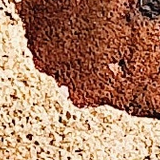
\includegraphics[scale=0.3]{realbrick1.png}\hspace{5px}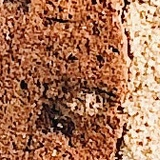
\includegraphics[scale=0.3]{realbrick2.png}\hspace{5px}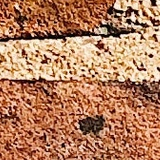
\includegraphics[scale=0.3]{realbrick3.png}\hspace{5px}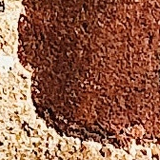
\includegraphics[scale=0.3]{realbrick4.png}\hspace{5px}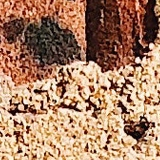
\includegraphics[scale=0.3]{realbrick5.png}\hspace{5px}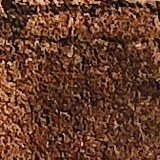
\includegraphics[scale=0.3]{realbrick6.png}\\
	\vspace{0.1cm}
	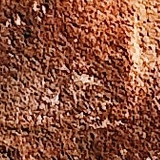
\includegraphics[scale=0.3]{realbrick7.png}\hspace{5px}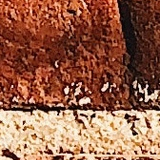
\includegraphics[scale=0.3]{realbrick8.png}\hspace{5px}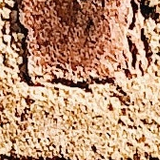
\includegraphics[scale=0.3]{realbrick9.png}\hspace{5px}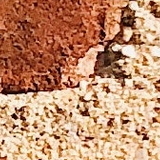
\includegraphics[scale=0.3]{realbrick10.png}\hspace{5px}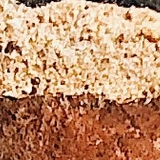
\includegraphics[scale=0.3]{realbrick11.png}\hspace{5px}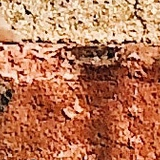
\includegraphics[scale=0.3]{realbrick12.png}\\
	
	Texture: Generated samples\\
	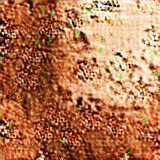
\includegraphics[scale=0.3]{brick1.png}\hspace{5px}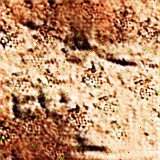
\includegraphics[scale=0.3]{brick2.png}\hspace{5px}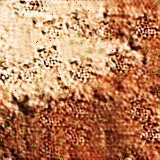
\includegraphics[scale=0.3]{brick3.png}\hspace{5px}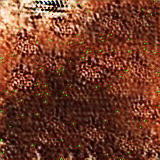
\includegraphics[scale=0.3]{brick4.png}\hspace{5px}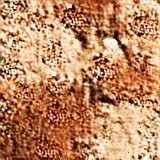
\includegraphics[scale=0.3]{brick5.png}\hspace{5px}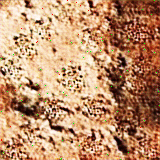
\includegraphics[scale=0.3]{brick6.png}\\
	\vspace{0.1cm}
	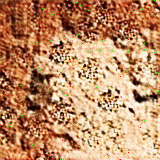
\includegraphics[scale=0.3]{brick11.png}\hspace{5px}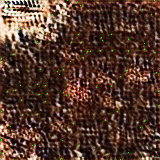
\includegraphics[scale=0.3]{brick12.png}\hspace{5px}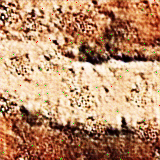
\includegraphics[scale=0.3]{brick13.png}\hspace{5px}\includegraphics[scale=0.3]{brick14.png}\hspace{5px}\includegraphics[scale=0.3]{brick15.png}\hspace{5px}\includegraphics[scale=0.3]{brick16.png}\\
	
	\caption{Real and generated samples from the Texture dataset.}
	\label{fig:samples_texture}
\end{figure}
\begin{figure}
	\centering
	CelebA: Real samples\\
	\includegraphics[scale=0.75]{realceleba_1.png}\hspace{5px}\includegraphics[scale=0.75]{realceleba_2.png}\hspace{5px}\includegraphics[scale=0.75]{realceleba_3.png}\hspace{5px}\includegraphics[scale=0.75]{realceleba_4.png}\hspace{5px}\includegraphics[scale=0.75]{realceleba_5.png}\hspace{5px}\includegraphics[scale=0.75]{realceleba_6.png}\\
	\vspace{0.1cm}
	\includegraphics[scale=0.75]{realceleba_7.png}\hspace{5px}\includegraphics[scale=0.75]{realceleba_8.png}\hspace{5px}\includegraphics[scale=0.75]{realceleba_9.png}\hspace{5px}\includegraphics[scale=0.75]{realceleba_10.png}\hspace{5px}\includegraphics[scale=0.75]{realceleba_11.png}\hspace{5px}\includegraphics[scale=0.75]{realceleba_12.png}\\
	
	CelebA: Generated samples\\
	\includegraphics[scale=0.75]{celeba_1.png}\hspace{5px}\includegraphics[scale=0.75]{celeba_2.png}\hspace{5px}\includegraphics[scale=0.75]{celeba_3.png}\hspace{5px}\includegraphics[scale=0.75]{celeba_4.png}\hspace{5px}\includegraphics[scale=0.75]{celeba_5.png}\hspace{5px}\includegraphics[scale=0.75]{celeba_6.png}\\
	\vspace{0.1cm}
	\includegraphics[scale=0.75]{celeba_11.png}\hspace{5px}\includegraphics[scale=0.75]{celeba_12.png}\hspace{5px}\includegraphics[scale=0.75]{celeba_13.png}\hspace{5px}\includegraphics[scale=0.75]{celeba_14.png}\hspace{5px}\includegraphics[scale=0.75]{celeba_15.png}\hspace{5px}\includegraphics[scale=0.75]{celeba_16.png}\\
	
	\caption{Real and generated samples from the CelebA dataset.}
	\label{fig:samples_celeba}
\end{figure}

\subsubsection{Application to hydro-geology}
\label{subs:subsurface}

\begin{table}
	\centering
	\begin{tabular}{l c c c c c}
		\Bigrule
		Dataset &Model           & Best \ac{HOG} & Best \ac{MSE}& \ac{HOG} at & \ac{MSE} at \\
		&&& &  best \ac{MSE} & best \ac{HOG} \\
		\bigrule
		Subsurface &CGAN   & \textbf{2.92e-4} & 0.2505 & \textbf{3.06e-4}  & 1.1550 \\
		&Ours            & 4.31e-4 & \textbf{0.0325}& 5.69e-4 & \textbf{0.2853} \\
	\end{tabular}
	\caption[Evaluation of the trade-off between the visual quality of the respect of the constraints for the Subsurface dataset]{Evaluation of the trade-off between the visual quality of the generated samples and the respect of the constraints for the CGAN approach and ours on the Subsurface dataset.}
	\label{tab:subsurface}
\end{table}

\begin{table}[t]
	\centering
	\begin{tabular}{l c c c c c}
		\Bigrule
		Dataset &Model           & Best \ac{HOG} &  \ac{MSE}& Best \ac{LBP} & Best \ac{LBP} \\
		&&& & (radius=1) & (radius=2) \\
		\bigrule
		Subsurface &CGAN   & \textbf{2.92e-4} & 0.2505 & \textbf{2.157} & \textbf{3.494}\\
		&Ours            &  4.31e-4 &\textbf{0.0325} & 10.142 & 16.754 \\

	\end{tabular}
	\caption[Evaluation of the visual quality on the Subsurface dataset]{Evaluation of the visual quality between the CGAN approach and ours on the Subsurface dataset using several metrics.}
	\label{tab:subsurface_visual}
\end{table}

Finally, we evaluate our approach on the Subsurface dataset. We use the UNetResPAC  architecture, since it performed the best on Texture data as exposed in Section \ref{sub:fcnn}. As previously, we simply set the regularization parameter at $\lambda=1$ and, the network is trained for 40 epochs using the same experimental protocol. To evaluate the trade-off between the visual quality and the respect of the constraints, instead of FID we rather compute distances between visual Histograms of Oriented Gradients (see Section \ref{sec:experiments_protocol}), extracted from real and generated samples. We also evaluate the visual quality of our approach with a distance between Local Binary Patterns. Indeed, Subsurface application lacks labeled data in order to learn a deep network classifier from which the FID score can be computed. 

%As stated before in Section \ref{subs:eval}, we cannot use the FID to evaluate the visual quality of the generated images since we don't have a supervised task linked to the data.
%Therefore we use distances between visual features, namely Histograms of Oriented Gradients and Local Binary Patterns (see Section \ref{sec:experiments_protocol}), extracted from real and generated samples.

The obtained results are summarized in Tables \ref{tab:subsurface} and \ref{tab:subsurface_visual}. They are coherent with the previous experiments since the generated samples are diverse and have a low error regarding the constrained pixels. The conditioning have a limited impact on the visual quality of the generated samples and compares well to unconditional approaches \citep{Ruffino2017}. Evaluation of the generated images using the domain-connectivity function highlights this fact on Figure \ref{fig:ours_connectivity} in the supplementary materials. Also examples of generated images by our approach  pictured in Figure \ref{fig:samples_subsurface} show that we preserve the visual quality and honor the constraints.

\begin{figure}[t]
	\centering
	Subsurface: Real samples\\
	\includegraphics[scale=0.3]{realchannel1.png}\hspace{5px}\includegraphics[scale=0.3]{realchannel2.png}\hspace{5px}\includegraphics[scale=0.3]{realchannel3.png}\hspace{5px}\includegraphics[scale=0.3]{realchannel4.png}\hspace{5px}\includegraphics[scale=0.3]{realchannel5.png}\hspace{5px}\includegraphics[scale=0.3]{realchannel6.png}\\
	\vspace{0.1cm}
	\includegraphics[scale=0.3]{realchannel7.png}\hspace{5px}\includegraphics[scale=0.3]{realchannel8.png}\hspace{5px}\includegraphics[scale=0.3]{realchannel9.png}\hspace{5px}\includegraphics[scale=0.3]{realchannel10.png}\hspace{5px}\includegraphics[scale=0.3]{realchannel11.png}\hspace{5px}\includegraphics[scale=0.3]{realchannel12.png}
	
	Subsurface: Generated samples\\
	\includegraphics[scale=0.3]{channel1.png}\hspace{5px}\includegraphics[scale=0.3]{channel2.png}\hspace{5px}\includegraphics[scale=0.3]{channel3.png}\hspace{5px}\includegraphics[scale=0.3]{channel4.png}\hspace{5px}\includegraphics[scale=0.3]{channel5.png}\hspace{5px}\includegraphics[scale=0.3]{channel7.png}\\
	\vspace{0.1cm}
	\includegraphics[scale=0.3]{channel11.png}\hspace{5px}\includegraphics[scale=0.3]{channel12.png}\hspace{5px}\includegraphics[scale=0.3]{channel13.png}\hspace{5px}\includegraphics[scale=0.3]{channel14.png}\hspace{5px}\includegraphics[scale=0.3]{channel15.png}\hspace{5px}\includegraphics[scale=0.3]{channel16.png}\\
	
	\caption{Real and generated samples from the Subsurface dataset.}
	\label{fig:samples_subsurface}
\end{figure}

\section{Conclusion and perspective}

\begin{figure}[!t]
	
	\begin{subfigure}[t]{0.5\textwidth}
		\centering
		\includegraphics[scale=0.5]{Gaussian}
		\caption{Gaussian best fit}
		\label{fig:rec_error}
	\end{subfigure}\begin{subfigure}[t]{0.5\textwidth}
		\centering
		\includegraphics[scale=0.5]{Mixture}
		\caption{Mixture distribution fit}
		\label{fig:mixture_dist}
	\end{subfigure}	
	\caption[Better modeling of the reconstruction error on the Subsurface dataset]{In orange: Histogram of the reconstruction error of the UNetResPAC model on 100 generated subsurface images, with $\lambda = 1$. As we can see, the error is either close to 0, -2 or 2. In blue: Probability density functions of a best fit Gaussian and a mixture model of a Gaussian distribution with a weight of 0.95 and two exponential distribution, each with weights of 0.025 (0.05 being roughly the error rate of the UNetResPAC model).}
\end{figure}

In this chapter, we address the task of learning effective generative adversarial networks when only very few pixel values are known beforehand. To solve this pixel-wise conditioned GAN, we model the conditioning information under a probabilistic framework. This leads to the maximization of the likelihood of the constraints given a
generated image. Under the assumption of a Gaussian distribution over the given pixels, we formulate an objective function composed of the conditional GAN loss function regularized by a $\ell_2$-norm on pixel reconstruction errors. We describe the related optimization algorithm.

Empirical evidences illustrate that the proposed framework helps obtaining good image quality while best fulfilling the constraints compared to classical GAN approaches. We show that, even when including the PacGAN technique,  this approach  allows for the use of fully-convolutional architectures and scales well to larger images. We apply this approach to a common geological simulation task and show that it allows the generation of realistic samples which fulfill the prescribed constraints.


In future work, an interesting direction would be to investigate other prior distributions for the given pixels. As mentioned in the section \citesec{subs:maximum_a_posteriori}, we assume that the reconstruction error of the model is Gaussian. This however is not necessarily true in practice, as we observed that in the case of the Subsurface dataset, since the pixels are always either -1 or 1, the reconstruction error tend to be close to either 0, -2, or 2 (see \citefig{fig:rec_error}). For this example, a mixture distribution could be more appropriate as it could model both the cases where the error is close to 0 (which can be assumed to be normal) and the cases where it is close to -2 or 2 (\citefig{fig:mixture_dist}). 

On the other hand, applying the developed approach to other applications or signals such as audio inpainting \citep{Marafioti2018} could also be an interesting perspective. Domains in which measuring points in any signal is costly or very noisy could benefit from an approach that allows fast sampling of potential solutions.
